%%%%%%%%%%%%%%%%%%%%%%%%%%%%%%%%%%%%%%%%%%
%Copyright (C) 2018-2019 YuZJ Lab.
%使用CC-BY-NC-SA授权。一份完整版本的许可证已位于附录。这个版本原始作者YuZJ,
%邮箱\theafamily@126.com(最后连接于2019年06月20日17:32:17)。
%%%%%%%%%%%%%%%%%%%%%%%%%%%%%%%%%%%%%%%%%%
\documentclass{book}
\usepackage{xeCJK} %中文支持
\setCJKsansfont{SourceHanSansCN-ExtraLight.otf}
\setCJKmonofont{SourceCodePro-Light.otf}
\setCJKmainfont{SourceHanSerifSC-ExtraLight.otf}
\setCJKfamilyfont{bolded}{SourceHanSansSC-Bold.otf}
\renewcommand{\bf}{\CJKfamily{bolded}}  
\newcommand{\normalall}{\normalsize\normalfont\normalcolor}  
\usepackage{color}
\usepackage{graphicx}  %生成图片
\usepackage{geometry} %设置页面排版
\geometry{top=0.5in, bottom=0.5in, left=0.5in, right=0.5in, papersize={21cm,29.7cm}}
\usepackage[super]{nth} %生成序数词
\bibliographystyle{unsrt}
\usepackage{metalogo} %生成TeX标志
\usepackage{texnames} %生成TeX标志
\usepackage{fancybox} %生成带阴影的盒子
\shadowsize=2pt %配置盒子
\usepackage{shorttoc}
\usepackage{flafter}%使得所有浮动体不能被放置在其浮动环境之前
\usepackage{picinpar} %生成文本环绕
\usepackage{indentfirst}%生成段落
\usepackage[toc]{multitoc}%双栏目录
\makeatletter\renewcommand{\verbatim@font}{\footnotesize \color{blue}\texttt} \makeatletter%修改verbatim环境格式
 %生成章节中文名和盒子
\renewcommand{\thechapter}{\arabic{chapter}}
\renewcommand{\thesection}{\arabic{chapter}.\arabic{section}}
\renewcommand{\thesubsection}{\arabic{chapter}.\arabic{section}.\arabic{subsection}}
\renewcommand{\thesubsubsection}{\arabic{chapter}.\arabic{section}.\arabic{subsection}.\arabic{subsubsection}}
\usepackage{titlesec}
\renewcommand{\bibname}{参考文献}
\renewcommand{\contentsname}{目录}
\renewcommand{\appendixname}{附录}
\titleformat{\chapter}[frame]{\bf \Huge}{\small 第 \thechapter 部分}{0pt}{}
\titleformat{\section}[frame]{\bf  \LARGE}{\small 第 \thesection 章}{0pt}{}
\titleformat{\subsection}[frame]{\bf  \Large}{\small  第\thesubsection 节}{0pt}{}
\titleformat{\subsubsection}[frame]{\bf \large}{\small 第\thesubsubsection 小节}{0pt}{}
\linespread{1.2} %行距命令
\usepackage{eso-pic}%背景图像命令
\usepackage[backref]{hyperref} %生成书签,这个应被放在末尾
\hypersetup{hidelinks,bookmarks=true,bookmarksopen=true,pdftitle=电教委员完全(不)技术指南,pdfauthor=YuZJ Lab}
\begin{document}
\setcounter{tocdepth}{5}
\begin{titlepage}	
\AddToShipoutPictureBG*{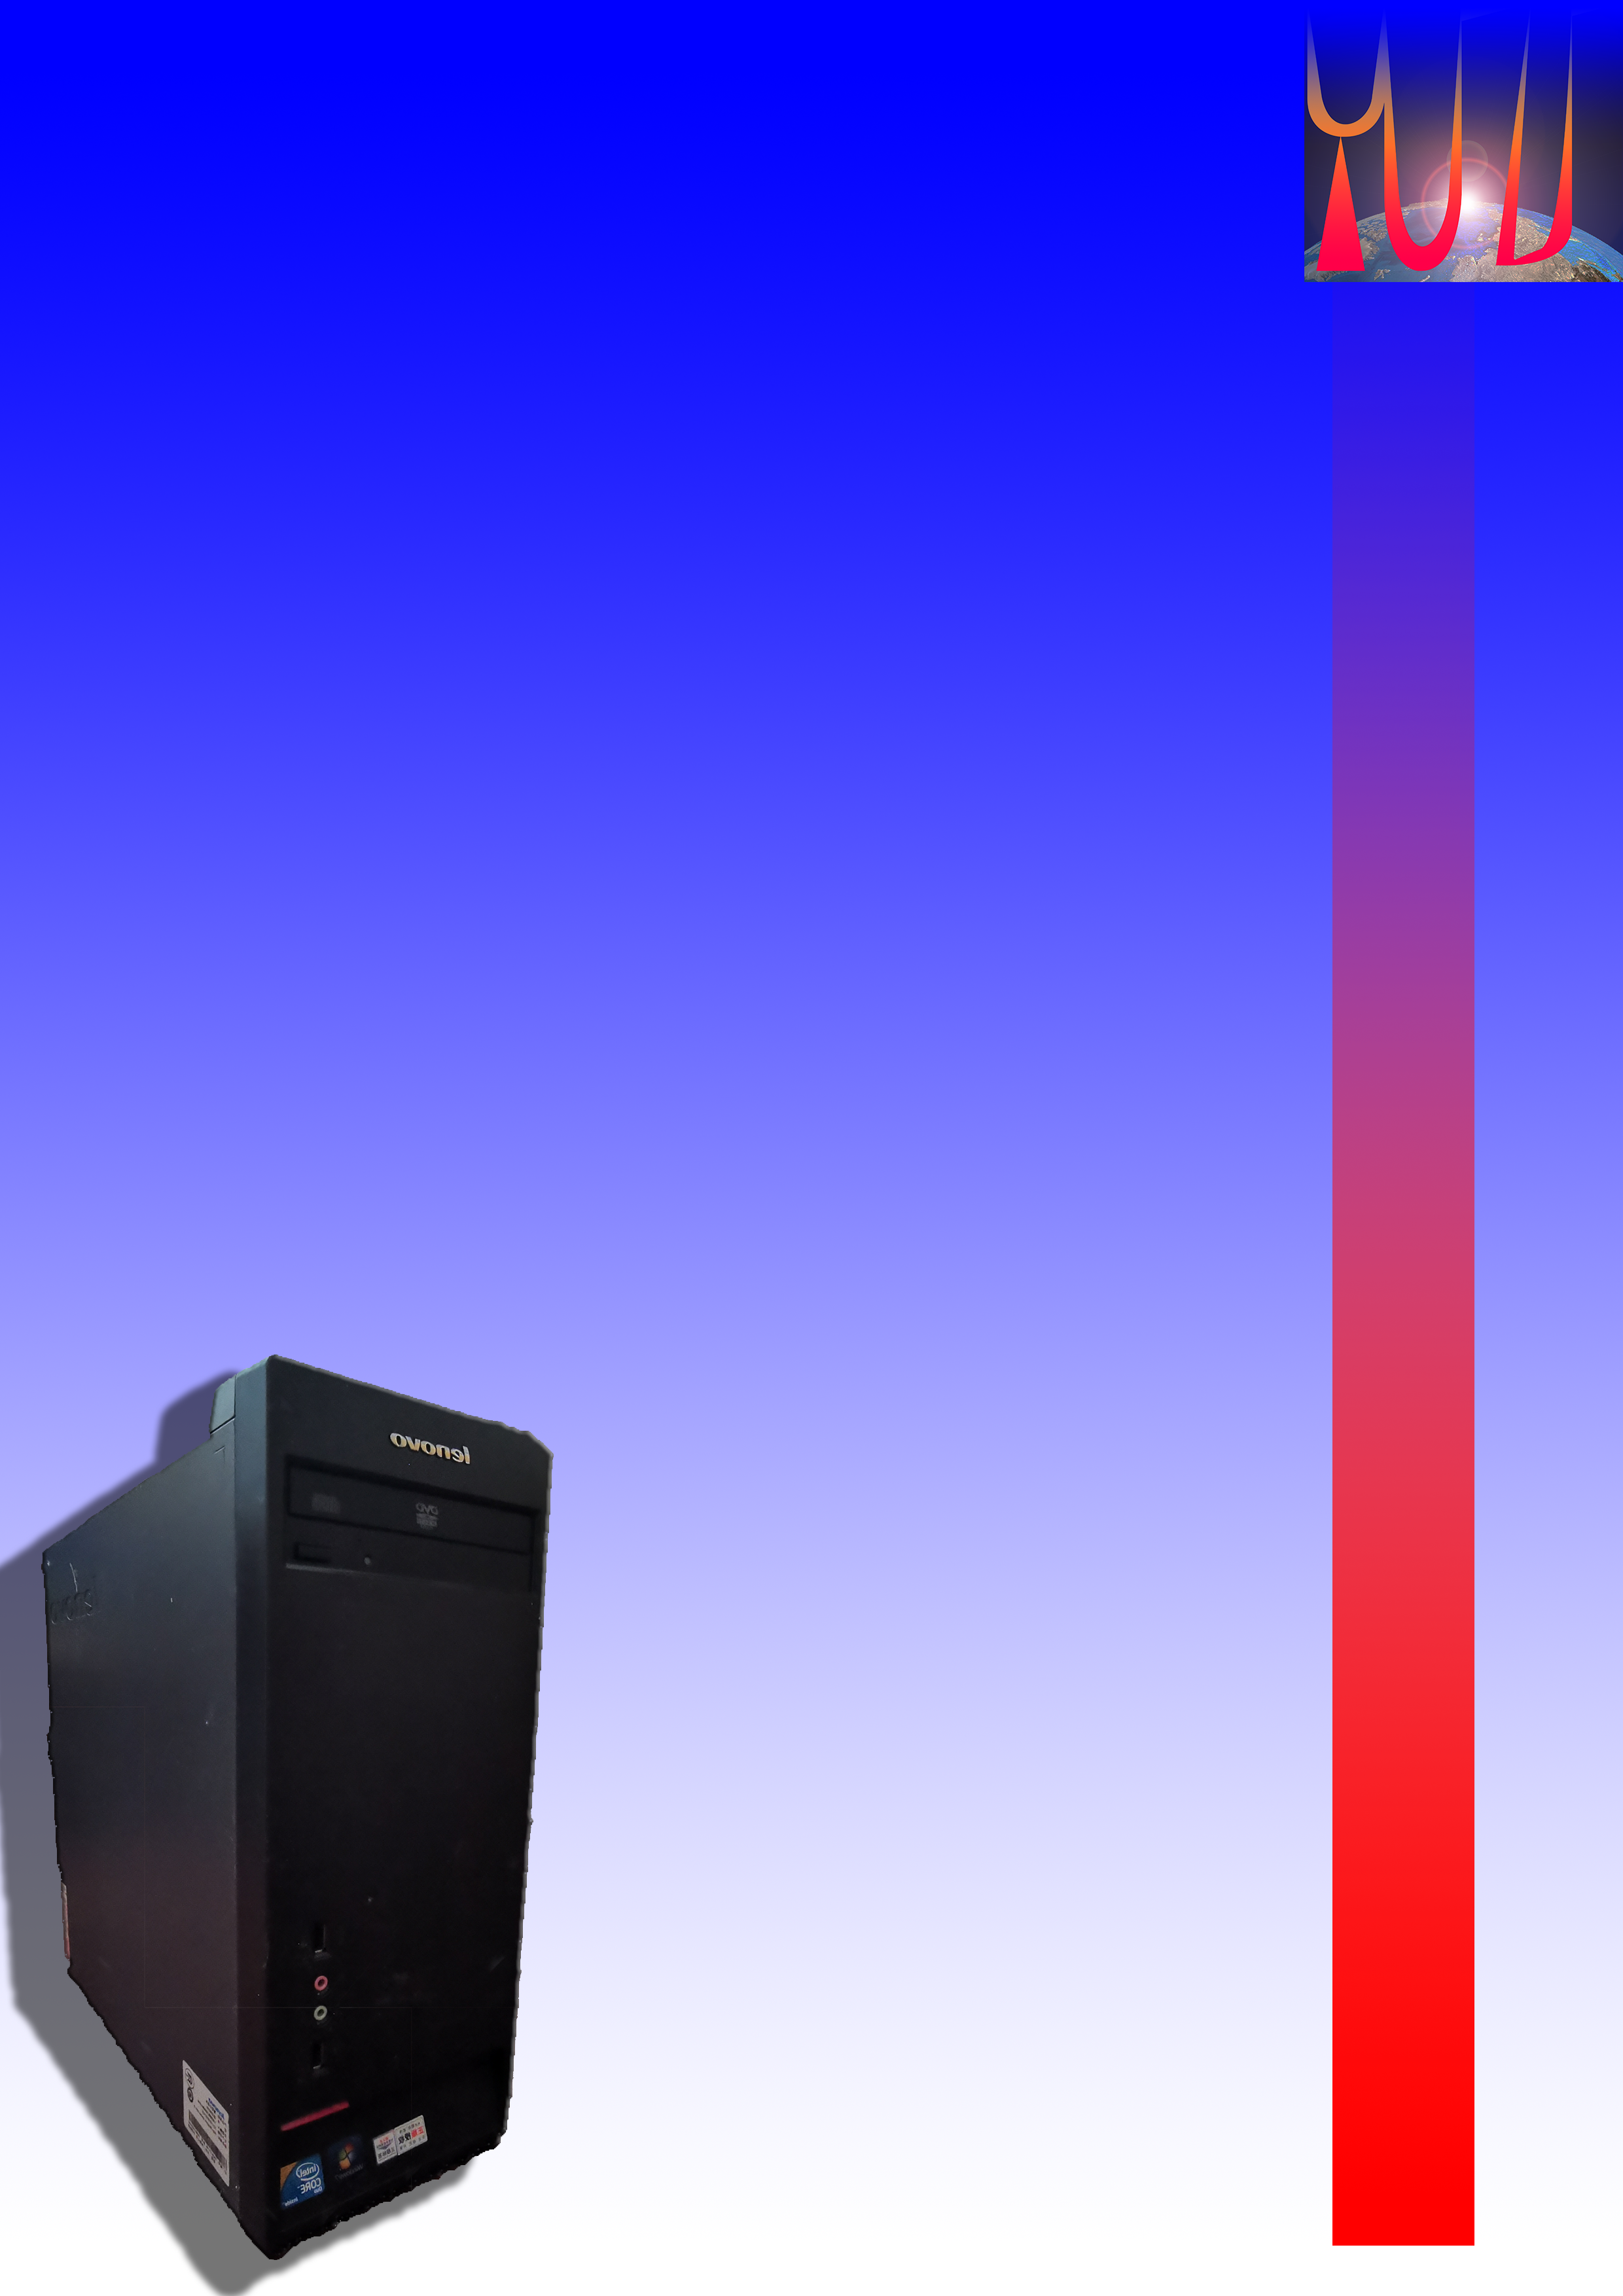
\includegraphics[width=21cm,height=29.7cm]{pic/face.png}}
{\color{white}{
\vspace*{10mm}
\begin{center}
\doublebox{\parbox{18cm}{
\begin{center}	
\Ovalbox{\Huge \bf 电教委员(不)完全技术指南(简体中文)\normalsize}\\\vspace*{5mm}\bf \large 作者:YuZJ Lab \\\vspace*{5mm} 编译日期:\today	
\end{center}}}
\end{center}}}
\vspace*{25mm}\normalall
\shadowbox{\parbox[t]{8cm}{“工欲善其事,必先利其器”,对于我们来说,掌握如何高效率地使用计算机是十分重要的。为了方便信息化教学的开展,我结合自己的工作经历,不自量力地“年来著书一种”,为希望掌握关于如何高效地使用教室计算机的初级和高级技巧的电教委员或者其余希望提高计算机技能的教师、学生及其他教职人员编写了这份文件。通过对自由/开源与专有软件的论证,我希望能够引导学生形成他们的软件价值观。}}
\end{titlepage}
\begin{center}
	\Huge \bf 试行本 \normalall
\end{center}
\shorttoc{简明目录}{1}
\tableofcontents
\chapter{在开始之前}
%%%%%%%%%%%%%%%%%%%%%%%%%%%%%%%%%%%%%%%%%%
%Copyright (C) 2018-2019 YuZJ Lab.
%使用CC-BY-NC-SA授权。一份完整版本的许可证已位于附录。这个版本原始作者YuZJ,
%邮箱theafamily@126.com(最后连接于2019年06月20日17:32:17)。
%%%%%%%%%%%%%%%%%%%%%%%%%%%%%%%%%%%%%%%%%%
\chapter{在开始之前}
\section{Copyright 版权}
Copyright \copyright{} 2018-2019 YuZJ Lab. \par
使用CC-BY-NC-SA授权。一份完整版本的许可证已位于附录。这个版本原始作者YuZJ,邮箱\url{theafamily@126.com}(最后连接于2019年06月20日17:32:17)。
\begin{center}\large \bf {\color{red}{对本文档所引起的任何后果不作担保!}}\normalall\end{center}
\section{序}
首先声明一下:在这里提及非自由软件并非我的意愿。作为自由软件的支持者,我当然希望你们使用自由软件。但技术所限,非自由的内容不得不被包括在内。\par
《天工开物·序言》描述当时人们在生产方面的创造时写道:“天覆地载,物号数万,而事亦因之,曲成而不遗。”人类在计算机技术上的创造亦是如此。很高兴生活在信息时代(也许马上应改为“数据时代”),国内外优秀的软件都可以被免费或付费地获取以为我们所用。然而“工欲善其事,必先利其器”,对于我们来说,掌握如何高效率地使用计算机是十分重要的。如一位数学教师可用\LaTeX\footnote{\LaTeX 是一个产生于 \TeX 的一个排版系统。它在编辑公式方面十分强大(使用 \AmSTeX 等宏包 ),并且能够胜任巨型文档和复杂的排版任务(如交叉引用、创建索引、管理参考文献资料等等)。它使用“LaTeX Project Public Li­cense (LPPL)”开放源代码,并拥有CTAN(综合的TeX档案库网络,拥有\LaTeX 近乎全部的宏包和使用教程,并存在多个镜像站如TUNA源)(【CTAN: Comprehensive TeX Archive Network】\url{https://www.ctan.org/},最后连接于2019年7月6日21:08:02)的管理组织与tug(\TeX 用户组:【TeX Users Group (TUG)】\url{http://www.tug.org/}(最后连接于2019年7月8日15:05:21))。做一点小小的说明:如果不喜欢完全使用鼠标来编辑公式,当编辑复杂公式时我更倾向于\LaTeX。\LaTeX 更多依赖键盘,但是不是一个所见即所得的软件。就像编写网页一样,你需要“编译”(Compile)\LaTeX 代码才能得到正确的文件。再做一点小小的说明,本文档就是用\LaTeX 编写的。}而不是MS Office \footnote{MS是Microsoft(微软)的缩写,MS Office 是微软公司发布的非自由付费办公套件。相对于\LaTeX ,它最大的优点是所见即所得和具有图形界面。} 来高效地编辑公式或使用Git\footnote{一个高效的分布式版本控制软件。官方网站\url{https://git-scm.com/}(最后连接于2019年7月6日21:06:04)。}管理自己的论文。因此,为了方便信息化教学的开展,我结合自己的工作经历,不自量力地“年来著书一种”,为希望掌握关于如何高效地使用教室计算机的初级和高级技巧的电教委员或者其余希望提高计算机技能的教师、学生及其他教职人员编写了这份文件。\par
手册中题为“入门”的章节是针对初学者的\footnote{我指的是毫无基础的初学者——你甚至根本都不需要知道什么是“操作系统”。},它大致介绍了Windows操作系统和MS Office等软件来实现日常教学,Windows操作系统的简单技巧与最基础的Windows安全。题为“进阶”的章节是针对已有一定技能基础并希望尝试更加有效的Windows安全工具(如使用以GNU/Linux\footnote{应该使用“GNU/Linux”而不是“Linux”。请参见【Richard Stallman之GNU/Linux问答】\url{https://www.gnu.org/gnu/gnu-linux-faq.html}(最后连接于2019年06月20日17:32:59)。关于GNU/Linux的详细介绍参见\pageref{sec:gnulinux}页\ref{sec:gnulinux}。}为操作系统的反病毒光盘清除计算机病毒)的电教委员的。题为“高级”的章简单地节介绍了GNU/Linux 操作系统的一部分入门知识及其教学实现。\par
在介绍多种多样的软件时,我遵循的原则是法律——性能——易用性——价格。在性能相同的情况下,易用性优先(大多是专有软件),但我也不会忘了推荐一些不错的自由免费软件以减少希望廉价使用正版软件者的开支。通过对自由/开源与专有软件的论证,我希望能够引导学生形成他们的软件价值观。这也是我在本书末尾附上《GNU GPL》的原因。\par
 在使用这份手册时,最重要的是实践。本人才疏学浅,文本中或许有(大量)错误,请广大读者不吝赐教。联系方式:\url{theafamily@126.com}(最后连接于2019年06月20日17:32:17)。如果文档中存在任何侵权之处,请按邮箱联系。一经确认,将立刻改正。“丐大业文人,弃置案头。此书于功名进取,毫不相关也。”\par
时己亥年肆月廿七日,西历2019年5月1日\par
慈溪YuZJ于家之书房
\section{致班主任}
\noindent 尊敬的班主任:\par
您好!\par
当你发现你的学生在看这本书时,您不用感到惊慌。本书不会包含任何有关逃避班主任的耳目来玩游戏或者任何类似的技术,也不会让学生沉迷于计算机无法自拔。本书的主要目的是培养能够熟练使用计算机的高级电教委员,我相信在这本书的帮助下,你会对他们的工作更加满意的。\par
这本书里的大部分操作(包括但不限于激活操作系统、激活部分软件、下载软件、更新操作系统以及反病毒软件病毒库)需要网络连接。这些网络连接虽然可以被以其他工作替代,但是这将大大增加电教委员的工作量。因此,在确保电教委员是一个品行优良、作风端正的人的前提下,请允许你的电教委员使用网络连接。如果你们班的学生都是自控能力极强的学生,您可以考虑对这台计算机开放互联网。这样您的学生查询英语单词能够更加方便,计算机系统也能时时保持最新。\par
如果你发现通过使用这本书您的电教委员的效率确实比以往高了不少,你也可以免费从网络上获得一本。我相信这本书中的某些章节对于提高您的生产力将会有所帮助。
\section{重要!预先警告}
第一,本书内所有网络链接在“最后连接时间”前均有效且已经过Norton Safe Web的Edge插件、Microsoft SmartScreen筛选器及卡巴斯基网络反病毒(包含于卡巴斯基免费版2019,病毒库更新时间为检测当天12:00)检测。 {\color{red}{注意,至少我坚持认为本书中提到的所有应用程序都应该从其官方网站或镜像源处下载。我们不推荐本书的使用者从任何非官方软件发布处下载任何本书中提到的软件(官方认可的镜像源除外)。}}\footnote{如腾讯电脑管家“软件中心”(提供过时的软件,如“Avira Antivir Personal 个人免费版”。软件链接:\url{https://pc.qq.com/detail/19/detail_819.html}(最后连接于2019年7月29日16:02:42),软件的发布日期为2016-11-14,最新版本发布日期应该已经是2019了。)或PC6等下载站。}。\par 
第二,从任何网站下载“破解版”或“注册机”“算号器(KeyGen)”“KMS注册机(这里仅指非法的KMS服务器。合法的服务器不用担心)”(以下简称“侵权程序”)都是不被允许的。这些侵权程序大部分含有“后门”或直接携带病毒(主要表现为网络蠕虫、挖矿机程序和Rootkit,或皆有)。具体请参见:
\begin{enumerate}
	\item 【“小马激活”病毒日感染数万台电脑 建议百度、360屏蔽该关键词】\url{https://www.huorong.cn/info/146173867117.html}
	\item 【火绒安全警报:病毒伪装成激活工具  强制安装360、2345浏览器】\url{https://www.huorong.cn/info/1535631707148.html}
	\item 【“小马激活”病毒新变种分析报告】\url{https://www.huorong.cn/info/146173922919.html}
	\item 【激活工具带毒感染量近60万 北京等四城市用户不被攻击】\url{https://www.huorong.cn/info/1526627586130.html}
	\item 【火绒安全-下载站行业乱象:流氓软件和电脑病毒重灾区】\url{https://www.huorong.cn/info/149181215360.html}
\end{enumerate}\par
对于错误反馈,任何由于违反以上两条原则导致的问题将不会被回复。\footnote{以下为对原文中重要内容的引用。火绒工程师认为:所谓的“下载器”和“高速下载通道”既没有用处,也没有存在的必要。为了躲避这些“下载器”的侵扰,用户可以去某个软件的官网下载产品,一般不用担心下载到下载器。这些“下载器”存在的意义就是为了捆绑安装其他软件。这些捆绑软件无一例外都不是用户当时想要的,如果想要这些软件,在下载站上都能找到。总之,除了给用户制造麻烦,所谓这些“高速下载通道”和“下载器”没有任何作用。}\par 
如果你确信你的下载站提供了可靠的软件,你也需要使用哈希校验来确保文件可靠性。方法:使用7Zip在文件资源管理器中的右键菜单“CRC SHA”选项校验哈希值并于官方提供的哈希制作比较。如果一致,那么这个软件可视为是官方的。 \par
第三,本书所有操作都是基于硬盘启动(而不是网络启动)的计算机,请先检查一下硬盘并与电教员联系。\par 
第四,请注意在安装任何软件时查看最终用户许可声明(EULA)和隐私协定!这将让你了解软件的使用条例。经验主义和机会主义者在将会付出代价。
\begin{center}\Large \bf {\color{red}{本书将不会提供任何有关破解专有软件的方法\\或进行反向工程、反向汇编、反向编译的知识。}}\normalall\end{center}
经检测的镜像站列表如下(检测于2019年6月22日17:16:47):
\begin{description}
	\item [【清华大学开源软件镜像站 | Tsinghua Open Source Mirror】]\url{https://mirrors.tuna.tsinghua.edu.cn/}
	\item [【USTC Open Source Software Mirror】]\url{http://mirrors.ustc.edu.cn/}
	\item [【欢迎访问网易开源镜像站】]\url{http://ubuntu.cn99.com/}\url{http://mirrors.163.com/}
	\item [【华为开源镜像站\_软件开发服务\_华为云】]\url{https://mirrors.huaweicloud.com/}
	\item [【阿里巴巴开源镜像站】]\url{https://opsx.alibaba.com/mirror}
	\item [【兰州大学开源社区镜像站】]\url{http://mirror.lzu.edu.cn/}
	\item [【重庆大学开源软件镜像站 | Chongqing University Open Source Mirror Site】] \url{https://mirrors.cqu.edu.cn/}
	\item [【Nanjing University Open Source Mirror Site】] \url{https://mirrors.nju.edu.cn/}
	\item [【南京邮电大学开源软件镜像站 | Njupt Open Source Mirror】]\url{https://mirrors.njupt.edu.cn/}
	\item [【Mirrors@NWAFU】]\url{https://mirrors.nwafu.edu.cn/}
	\item [【这个似乎是搜狐的......具体叫什么我也不清楚】]\url{https://mirrors.sohu.com/}
	\item [【SourceForge - Download, Develop and Publish Free Open Source Software】] \url{https://sourceforge.net/}
	\item [【FOSSHUB】] \url{https://www.fosshub.com/}
	\item [【The world’s leading software development platform · GitHub】] \url{https://github.com/}
\end{description}
\section{自由软件、开源软件和专有软件}
我们以是否公开源代码为标准来区分一个软件是不是专有软件。不公开源代码(你只能得到可执行文件(参见\pageref{sec:exe}页的\ref{sec:exe}))的软件称为“专有软件”,而公开源代码的软件称为开源或者自由软件。我们以许可证是否兼容《GNU General Public License v3》(《GNU通用公共授权第3版》)来确定这个软件是否自由,如果兼容即为自由软件。一个软件在安装时就会展示许可证(如下图为安装Filezilla时展示的GNU GPL许可证),你应该仔细地阅读它并决定是否安装。
\begin{center}
	\includegraphics[scale=0.6]{pic/fzi}
\end{center}\par
源代码允许用户“自由”使用的软件称为自由软件。然而“自由”是一个很难定义的名词,因此我们使用Richard Stallman的标准界定“自由”。请参见【Various Licenses and Comments about Them - GNU Project - Free Software Foundation】\url{http://www.gnu.org/licenses/license-list.html}(最后连接于2019年07月30日18:08:02)来确定你的许可证是否自由。\par
哪些是专有软件?我们日常所用的软件(如Windows操作系统、Office办公软件、QQ、微信与Photoshop等等),基本上全都是专有软件。\par
我虽然支持自由软件,但是承认拥有\bf 合法版权\normalall 的专有软件的合法性。在这本书中,在\bf 不影响使用\normalall 的前提下如果能完成此功能的专有软件能被自由/开源软件替代,我将使用后者。以下是一些常见问题的解答。
\subsection{为什么本书不使用《GNU GPL》或其它GNU的协议?}
\begin{enumerate}
	\item 第12款规定:“If conditions are imposed on you (whether by court order, agreement or otherwise) that contradict the conditions of this License, they do not excuse you from the conditions of this License.”(意为“即便你面臨與本協議條款衝突的條件(來自於法庭要求、協議或其他),那也不能成為你違背本協議的理由。”)
	\item 2.序言规定:For the developers' and authors' protection, the GPL clearly explains that there is no warranty for this free software. (意为“為了保護每一位作者和開發者,GNU通用公共授權合約指明一點:自由軟體並沒有品質擔保。”)
	\item 存在一些其他的表述不清以及前后矛盾问题。
	\item 我不希望这本书被运用于商业用途,而《GNU FDL》并没有禁止对商业用途的使用。
\end{enumerate}
\subsection{那么,使用自由/开源软件有什么好处?}
首先是价格。请注意,我没有在道德层面上批判收费行为——无论是专有软件还是自由软件的创造者都有权利因\bf 自己的\normalall 创造得到物质上与精神上的回报。自由软件大多数是免费的,收费的开源软件也不多,但功能强大的专有软件大部分收费。\par
其次是安全性。(除了自由社区研究使用的病毒程序以外)显然地,自由/开源软件敢于将代码和开发过程(指源代码的版本控制机制,任何对源代码的修改一经保存都可以被查到)示人,就说明他们有勇气接受全世界软件开发者和用户,尤其是他的竞争对手等人的监督。自由软件敢承诺没有任何恶意代码或者后门。专有软件的代码不开放性决定了恶意代码或“后门”能被非常方便地置入代码中。这种恶意代码不是专业的开发者是无法发现的,而发现此类问题的专业的开发者则有可能受制于政治、经济或法律因素无法曝光此类问题(一个程序员怎么可能与训练有素的律师团队对抗?)。除此之外,一小部分专有软件(尤其是某些手机APP)都会收集大大超过他们需求的个人信息,这是我们普通消费者出来拒绝使用以外无法阻止的。\par
最后是自由软件更新发布速度。自由软件的开发是分布式的,一旦出现任何漏洞,一定会在漏洞散布之前被全世界的程序员修补。专有软件和开源软件大多数是一家公司集中开发的,如果出现问题几乎只能依靠公司解决。
\subsection{那么,为什么自由/开源软件还不流行?}
开发上,“社群”等其它去中心化的组织方式决定了自由/开源软件生产者内部也会因为意见不同(或者价值观不同——比如说GPL阵营与BSD阵营)而引发争端,专业/非专业的开发并存也是整个自由/开源软件界存在的问题。\par
使用上,自由软件相较于能实现相同功能的专有软件操作一般较为繁琐(如LibreOffice与MS Office,GIMP与Photoshop,GNU/Linux与Windows。当然这一点见仁见智)并声明“不提供品质担保”,这使自由软件的使用者局限于专业领域从业人员而不是大众。自由软件在宣传上显然也弱于专有软件。
\chapter{入门}
\input{Basic}
\chapter{进阶}
%%%%%%%%%%%%%%%%%%%%%%%%%%%%%%%%%%%%%%%%%%
%Copyright (C) 2018-2019 YuZJ Lab.
%使用CC-BY-NC-SA授权。一份完整版本的许可证已位于附录。这个版本原始作者YuZJ,
%邮箱theafamily@126.com(最后连接于2019年06月20日17:32:17)。
%%%%%%%%%%%%%%%%%%%%%%%%%%%%%%%%%%%%%%%%%%
\chapter{进阶}
\section{Windows操作系统上的高级反病毒技巧}
当一般的反病毒软件无法将病毒清除时,你就应该考虑使用GNU/Linux反病毒\footnote{当然你也可以重装系统。但这么做无法清除系统盘以外的病毒。}。
\subsection{使用以GNU/Linux为操作系统的计算机急救工具}
GNU/Linux可用于Windows反病毒原因是:Windows二进制文件与GNU/Linux二进制文件的结构是不同的(具体请参考其他专业书籍),因此Windows的EXE病毒大多数情况下无法在GNU/Linux上运行(使用Wine \footnote{一种类似于虚拟机的技术,它可允许Windows应用程序在GNU/Linux,BSD等操作系统上运行。} 或其他类似技术除外),也就是说,Windows下的病毒一般无法感染GNU/Linux操作系统。\par
大多数反病毒软件厂商都提供了“急救盘”,用于给无法启动或严重感染的计算机反病毒。大多数急救盘基于GNU/Linux \footnote{如Dr.Web和AVIRA基于Ubuntu 14(Dr.Web凭借Wine运行),Kaspersky基于Gentoo Linux x86\_64,ESET基于其它GNU/Linux操作系统。},也有少部分(如Avast!)基于Windows。\par
现将以Kaspersky Rescure Disk以演示GNU/Linux反病毒。至于如何安装GNU/Linux并反病毒请参见\pageref{sec:avgl}页\ref{sec:avgl}\par
现在你将计算机开启,将光盘插入光驱后重启。你将被引导到光盘启动。你将发现:
\begin{center}
	\includegraphics[scale=0.7]{pic/krd1}
\end{center} \par
此时,快速按下ESC键(它应位于你键盘左上角),进入左图所示界面,选择“English”--英语,敲击回车,进入右图界面。此时你应该选择“Kaspersky Rescure Disk, Graphic Mode”(图形界面)\footnote{下面“Limited graphic mode”为限制的图形界面,“Hardware info”为探测硬件信息,“Boot from hard disk”为从硬盘启动(意思就是说,启动硬盘里已经安装的操作系统),“Reboot”与“Shutdown”指重启与关机。当然高手请随意。}
\begin{center}
	\includegraphics[scale=0.25]{pic/krd2}	\includegraphics[scale=0.25]{pic/krd3}\\
	\includegraphics[scale=0.35]{pic/krd4}	\includegraphics[scale=0.35]{pic/krd5}
\end{center} \par
这就启动好了。KRD提示你整个系统正在内存上运行,所有新病毒库、日志、隔离等在关机后都将丢失。之后你会看见右图界面:我们使用卡巴斯基病毒移除工具(Kaspersky Virus Removal Tool,KVRT)演示它们的使用。下载:\url{https://www.kaspersky.com.cn/downloads/thank-you/free-virus-removal-tool}(最后连接于2019年06月20日18:44:31,网速较慢)。
\begin{center}
	\includegraphics[scale=0.5]{pic/kvrt_eula.PNG}        \includegraphics[scale=0.6]{pic/kvrt_ready.PNG}\\
	\includegraphics[scale=0.6]{pic/kvrt_conf.PNG}
	\includegraphics[scale=0.4]{pic/kvrt_ing.PNG}    \includegraphics[scale=0.4]{pic/kvrt_compl.PNG}
\end{center} \par
上图分别是KVRT显示最终用户许可声明及隐私保护条例,准备查杀,配置扫描范围,正在查杀,查杀完成的界面。\par
首先你应该同意最终用户许可声明及隐私保护条例(注意,你首先应该看过它)。选中两个复选框再单击“Accept”即可。之后它会“初始化”(initialization)一段时间,并显示“准备好”界面。注意到上面黄色的一块区域了吗?它的出现说明这个版本已经过时了,你可以选择重新下载最新版。\par
现在选择查杀范围。单击“change parameters”,你将发现图3所示对话框。其中“System memory”指“系统内存”,“Startup objects”指启动项,“Boot sectors”指启动扇区,“System drive”指系统盘(一般是“C:\textbackslash”)。你还可以单击“Add object”添加其它文件或磁盘。单击“Start scan”开始扫描\footnote{需要消耗一(大)段时间并占用大量系统资源}。如果发现病毒,KVRT将在GNU/Linux下删除它们。
除了反病毒,KRD还提供了网络浏览器Firefox、终端、任务管理器Htop与Task Manager(参见\pageref{sec:pm}页\ref{sec:pm})、图像查看器Ristretto Imagine Viewer、文件管理器Midnight Commander与Thunar File Manager、文本编辑器Mousepad等。默认以root用户登录。其余设置较为复杂,请参照“高级”章。

\chapter{高级:GNU/Linux的教学实现}
\input{Advanced}
\appendix
\renewcommand{\thechapter}{\Roman{chapter}}
%%%%%%%%%%%%%%%%%%%%%%%%%%%%%%%%%%%%%%%%%%
%Copyright (C) 2018-2019 YuZJ Lab.
%使用CC-BY-NC-SA授权。一份完整版本的许可证已位于附录。这个版本原始作者YuZJ,
%邮箱theafamily@126.com(最后连接于2019年06月20日17:32:17)。
%%%%%%%%%%%%%%%%%%%%%%%%%%%%%%%%%%%%%%%%%%
\chapter{附录}
\section{跋}
在创作这本书的时候,我深深地感到了我语言的苍白、英语水平低下,对计算机知识的了解也仅仅浮于表面。我不得不对在计算机方面雄心勃勃的电教委员说,学好英语是第一要务。\par
“技”海无涯,这本书将永远“不”完全,并会不断完善下去。恳请广大读者不吝赐教。
\section{强大的生产力所需的网络架构:以Ubuntu Server 19.04为操作系统搭建服务器}
这一部分是针对电教员的。你需要安装一台具有固定IP(或者你可以让你的用户在每一次需要使用时打你的电话问一下当前服务器IP地址)的Ubuntu Server 19.04(或者其它类似的操作系统)。
\subsection{防火墙与固定IP}
若需要设置固定IP,请使用文本编辑器编辑“/etc/netplan/”目录下的一个扩展名为“yaml”的文件。你将得到:
\begin{verbatim}
1 # This file describes the network interfaces available on your system
2 # For more information, see netplan(5).
3 network:
4   version: 2
5   renderer: networkd
6   ethernets:
7     ##这里应该显示网卡名称。
8       addresses: [192.168.0.101/24]##IP地址及网络号长度(对应子网掩码255.255.255.0)
9       gateway4: 192.168.0.1##默认网关
10       nameservers:##DNS服务器
11         addresses: [8.8.8.8]
12
##前面的数字是Vim显示的行号。
\end{verbatim}\par
我们现在使用一款名为“ufw”的防火墙软件(从软件源里安装它)。ufw能够进行一些简单的网络设置。注意更改设置需要使用root权限。常用的命令如(具体请参照man手册):
\begin{verbatim}
ufw enable##开启ufw
ufw disable##关闭ufw
ufw allow in to 192.168.0.102##允许来自于192.168.0.102的进入。
##这个命令语法是“ufw [规则]”,上例中“allow in to 192.168.0.102”属于[规则]。
##这个规则语法是
[allow/deny/reject] proto [协议名] [in/out] on [网卡名] from [IP地址] to [IP地址]
##其它常见规则语法:
[allow/deny/reject][端口号]/[协议名,如TCP]
[allow/deny/reject][协议名,如SMTP]
##deny为禁止进入(丢弃传入的数据包),reject为拒绝进入(返回一个错误信息)。
ufw defaut [allow/deny/reject]##选择默认政策。
ufw logging [on/off]##是否使用日志。
ufw delete [规则]##删除规则。
\end{verbatim}
\subsection{-使用VSFTPD配置FTP服务器}
VSFTPD(非常安全FTP守护进程)是一个在GNU/Linux平台被广泛使用的ftp服务器。下面以Ubuntu Server 19.04为例教你如何使用VSFTPD。\par
案例背景:现在我们需要为教师配置FTP服务。教师都要有一个私有云盘(完全控制)和公用区域(仅下载)。我们还需要一个管理员账户管理所有的文件。
\subsubsection{配置文件系统:将FTP放在分别的磁盘上}
\begin{verbatim}
root@server:/etc#mkdir /var/ftp
##新建FTP根目录
root@server:/etc#cd /var/ftp
root@server:/var/ftp#chown root.root /var/ftp
##请注意,VSFTPD要求FTP根目录不可写。
root@server:/var/ftp#chmod a-w /var/ftp
root@server:/var/ftp#mkdir main
root@server:/var/ftp#chown ftplink.ftplink main
root@server:/var/ftp#chmod u+w+r+x /var/ftp/main
##建立可写目录main。
##/var/ftp/main/Public用于存放公共文件。
##/var/ftp/main/Private/[用户名]用于存放用户文件。
root@server:/j# chown root.root/etc/vsftpd*
root@server:/# chmod a-r-w-x /etc/vsftpd*
##保证VSFTPD配置文件不能被其它用户读取。
\end{verbatim}\par
\subsubsection{下载安装}
这个太显然了吧。
\begin{verbatim}
sgcomputers@server:~$sudo apt install vsftpd
Reading packagelists... Done
Building dependency tree
##以下省略一大堆内容。
Processing triggers for systemd (240-6ubuntu5.1) …
\end{verbatim}
\subsubsection{配置VSFTPD基础设置}
此时我建议你先使用“\verb|su|”命令切换到root账户。这能节省时间。目前我的VSFTPD最高版本为3.0.3,配置文件是“/etc/vsftpd.conf”。使用Vim或其它你喜欢的编辑器打开它,取消注释(删除“\verb|#|”)以下内容:
\begin{verbatim}
listen=YES
listen_ipv6=NO
anonymous_enable=NO
local_enable=YES
write_enable=YES
dirmessage_enable=YES
use_localtime=YES
xferlog_enable=YES
connect_from_port_20=YES
ascii_upload_enable=YES
ascii_download_enable=YES
allow_writeable_chroot=YES
anon_root=/var/ftp/
secure_chroot_dir=/var/vsftpd/empty
pam_service_name=vsftpd.vu
rsa_cert_file=/etc/ssl/certs/ssl-cert-snakeoil.pem
rsa_private_key_file=/etc/ssl/private/ssl-cert-snakeoil.key
ssl_enable=NO
guest_enable=YES
guest_username=ftplink
user_config_dir=/etc/vusers_dir
local_umask=022
userlist_enable=YES
tcp_wrappers=YES
\end{verbatim}
\subsubsection{配置VSFTPD认证设置}
为了验证用户,增加“/etc/pam.d/vsftp.vu”
\begin{verbatim}
auth required pam_userdb.so db=/etc/vuser
account required pam_userdb.so db=/etc/vuser
\end{verbatim}
\subsubsection{配置VSFTPD用户设置}
防止关键用户登录,添加“/etc/vsftpd.user\_list”
\begin{verbatim}
root
bin
daemon
adm
lp
sync
shutdown
halt
mail
news
uucp
operator
games
nobody
\end{verbatim}\par
现在配置虚拟用户。新建文件“/etc/vuser.list”,以一行用户名,一行密码方式添加。如:
\begin{verbatim}
01
01
02
02
\end{verbatim}\par
现在我们就有两个用户了。为了加密,我们使用这个命令:“\verb|db_load -T -t hash -f vuser.list vuser.db|”我们使用现在配置他们的权限。创建目录“/etc/vusers\_dir”,添加以用户名为文件名的文件。以“01”为例,应该是:
\begin{verbatim}
local_root=/var/ftp/main/Private/01
anon_umask=022
write_enable=YES
anon_mkdir_write_enable=YES
anon_upload_enable=YES
download_enable=YES
anonymous_enable=YES
anon_other_write_enable=YES
\end{verbatim}
现在以“ftplink”为例添加使用上述方法登陆的内建用户。这个内建用户是必须的。
\begin{verbatim}
root@server:/etc#useradd ftplink
##新建用户
root@server:/etc#passwd ftplink
##修改密码
Newpassword:
Retypenew password:
passwd:password updated successfully
root@server:/#mkdir /home/ftplink
\end{verbatim}\par
修改“/home/ftplink/.bashrc”文件,删除所有内容并添加
\begin{verbatim}
logout
exit
\end{verbatim}\par
来确保没人可以通过Telnet或SSH远程登录这个用户。

\subsubsection{调试}
\begin{verbatim}
root@server:/#service vsftpd start
\end{verbatim}\par
开始服务,现在请使用你喜欢的FTP客户端试验上传、下载、删除文件等操作吧。如果你需要配置多个用户,只需要重复这些操作就行了。注意你需要修改每个用户的目录权限并允许特定用户通过防火墙。
\subsection{在Windows下配置FTP服务器}
你不需要使用ServU,有一个自由免费的软件可以替代它——Filezilla Server。你不需要使用Windows Server(它的IIS已经可以搭建优秀的服务器了),一台具有固定IP的Winsows10即可!到它的官网上面下载安装吧!
\begin{center}
	\includegraphics[scale=0.6]{pic/fzs}
\end{center} \par
从上图中可以看到整个服务器是完全图形界面的。现在请跟我做:\par
1.打开防火墙。找到“控制面板”-“系统和安全”-“Windows Defender防火墙”-“允许应用通过Windows防火墙”,单击“更改设置”-“允许其他应用”,添加Filezilla Server(它应为于C:\textbackslash Program Files (x86)\textbackslash FileZilla Server\textbackslash FileZilla Server.exe)。“确定”保存。\par
2.现在开始配置服务器。双击图标进入服务器,对弹出框单击“Connect”(就是要连接本地服务器)。现在进入“Edit”-“Users”添加用户。在“General”页中单击“Add”添加用户和密码,在“Shared folders”页针对每一个用户添加目录和对应的权限即可。这样一个简单地FTP服务器就设置好了。
\subsection{使用Telnetd/SSHD配置远程登录服务器}
这太简单了,安装“telnetd”(CentOS是“telnet-server”)软件包并设置防火墙即可。
\subsection{使用SSHD与Git配置Git服务器}
现在将使用sshd与git配置git版本控制服务器。首先使用软件源安装这两个应用,设置好防火墙并使用“\verb|sudo service sshd start|”开启sshd服务。大部分命令与上一节创建FTP服务器类似,这里不再赘述。
\subsection{初始化}
先使用“\verb|useradd git|”新建用户“git”并修改密码,新建“/home/git/.ssh”目录并在里面创建“ authorized\_keys”文件。为了允许授权的用户访问服务器,请各位授权的用户运行“ssh-keygen”命令并将产生的“id\_rsa.pub”公钥文件发送到电教员手中(比如说,使用FTP),电教员将它们中的内容添加到“ authorized\_keys”文件末尾,一条公钥一行。\par
为了防止入侵,请修改“/etc/passwd”文件的“git”用户对应的一行末尾“/bin/bash”为“/usr/bin/git-shell”,使他大致呈现“git:x:xxxx:xxxx:xxx:/home/git:/usr/bin/git-shell”(某些内容用x表示)。
\subsection{创建仓库}
到“/opt/git”目录,使用“\verb|git init --bare --share [仓库名].git|”新建仓库并修改文件所有者为“git”并可读可写可执行,此时远程的用户就可以通过“\verb| git clone git@[服务器地址]:/opt/git/[仓库名].git|”来克隆这个仓库。未经授权的用户可以输入git用户的密码来访问。
\section{从此告别U盘}
我相信所有的电教员一定很反感U盘在教育教学中的使用:U盘不仅成为了病毒的“特快车道”,还有保密度低、容易遗失的不足。通过完善的网络配置即可除去U盘在教育教学中的使用。\par
首先,请使用硬件(这个太简单了吧,把线剪掉就好了)或软件(推荐这一种。可以使用火绒的相关功能)方法禁用学生机的USB接口。之后请搭建一个高速FTP服务器,确保每台教师机和学生机都能登录服务器。这样需要什么教学资源只要下载即可。或者也可以搭建无盘服务器,将教学资源放在服务器上。
\section{GNU宣言}
GNU宣言\footnote{我将这份历史文件添加进本技术指南的目的,是为了让程序员在商业化如潮水般推进时,能够关注一些其它理念。该份文件仅代表自由软件运动捍卫者的观点,并不能代表YuZJ Lab的观点或立场。\cite{gnum},被引用时文章内所有链接均有效。注意,有些脚注是由GNU CTT加的。}(如下所示)由\href{http://www.stallman.org/}{Richard Stallman}在1985年撰写,用来请求大家支持GNU操作系统的开发。其部分文本摘自1983年撰写的初始声明。直到1987年,因为开发的原因它时时小有更改;那时起,看起来最好是保持它不再改变。\par
时过境迁,我们认识到使用不同的措辞可以避免一些常见的误解。从1993年起,我们添加了脚注来澄清这些问题。\par
如果你想安装GNU/Linux系统,我们建议你使用\href{http://www.gnu.org/distros}{100\%自由的GNU/Linux发行版}之一。如果你想做出贡献,请参看\url{http://www.gnu.org/help/help.html}。\par
GNU工程是自由软件运动的一部分,该运动旨在\href{http://www.gnu.org/philosophy/free-sw.html}{捍卫软件用户的自由}。把GNU和“开源”一词联系在一起是错误的—该词汇是1998年由一些不赞同自由软件运动之道德价值的人士发明的。他们使用该词汇来推动同一领域的\href{http://www.gnu.org/philosophy/open-source-misses-the-point.html}{非道德方案}。\par
\subsection{GNU为何?GNU并非UNIX!}
GNU,代表的是Gnu's NotUnix(GNU并非UNIX),是我正在编写的一个完全兼容Unix的软件系统,这样我就可以把它自由地交给想要使用它的人。\footnote{此处用词不当。其初衷是人们不必为使用GNU系统而支付许可费。但是用词却没有清楚地说明此事,而人们经常理解为这是说GNU的拷贝总是免费或廉价地发行。这不是本意;后来,宣言指出公司提供有偿发行服务的可能性。之后,我也了解到认真区别自由中的“free(自由)”和价格中的“free(免费)”。自由软件是用户有自由修改和发布的软件。有些用户可能得到免费拷贝,而有些用户付费得到拷贝—如果这些资金帮助到软件的改善,善莫大焉。重要的一点是拥有拷贝的用户有自由和其他人一起使用自由软件。}还有几个志愿者在帮助我。我们非常需要大家在时间、金钱、程序和设备方面的贡献。\par
目前,我们有一个可以用lisp编写编辑命令的Emacs文本编辑器、一个源代码级别的调试器、一个兼容yacc的分析器生成工具、一个链接器和大约35个应用程序。shell(命令解释器)也接近完成。一个新的可移植的优化C编译器已经可以自我编译,可能会在年内发布。现有一个初始的内核,不过还需要增加很多功能才可以模拟Unix。当内核和编译器完成后,我们就有可能发布一个适合开发程序的GNU系统。我们会使用Tex作为文本排版工具,不过nroff还需要一些工作。我们还会使用自由的、可移植的XWindow系统。此后,我们还会加入一个可移植的CommonLisp、一个Empire游戏、一个电子表格和数百个应用以及在线文档。最终,我们希望提供Unix系统常规带有的一切有用之物,以及更多。\par
GNU将能够运行Unix的程序,但是它不完全和Unix一样。我们会根据我们在其他操作系统上的感受做出所有合理的改进。特别地,我们计划使用更长的文件名、文件版本号、防崩溃的文件系统、也许带有文件名填充、终端无关的显示支持、最后可能有一个基于Lisp的窗口系统,此时Lisp程序和普通Unix程序可以共享一个屏幕。C和Lisp都将作为系统编程语言。我们会支持UUCP、MITChaosnet和Internet等通信协议。\par
GNU最初的目标是68000/16000之类的带虚拟内存的机器,因为它们是最容易跑起来的机器。让GNU在更小的机器上运行的额外努力就留给那些需要使用这些机器的人吧。\par
为了避免可怕的混淆,请在指示本工程时,发出“GNU”中g的音。
\subsection{为什么我必须编写GNU}
我认可的黄金法则是如果我喜欢一个程序,我就必须把它分享给喜欢它的人。软件销售商通过让每个用户保证不和其他人分享来分化用户并控制他们。我拒绝以这种方式打破和其他用户组成的统一体。我的良知让我无法签署这样的保密协议或软件许可证协议。几年来,我在人工智能实验室都在反抗这种趋势以及其他冷漠,但是最终他们还是走得太远了:我无法再呆在一个为我做违背我意愿之事的机构。\par
为了能够继续不失颜面地使用计算机,我决定把一些必要的自由软件集合在一起,这样我就能够继续下去而不需要任何非自由软件。我从人工智能实验室辞了职,这样就可以在我发布GNU时避免和MIT产生法律纠葛。\footnote{2.“赠送”是另一个不妥的表达,它再次说明我那时还没有清楚地分开价格和自由的问题。我们现在建议在谈论自由软件时避免这一表达。请参看\href{http://www.gnu.org/philosophy/words-to-avoid.html\#GiveAwaySoftware}{“不清楚的词汇和短语”}了解更多解释}\par
\subsection{为什么GNU将会兼容Unix}
Unix并不是我理想中的系统,但是它还不算太差。Unix的主要功能看来是好的,而我认为我可以在不破坏这些好功能的情况下填补Unix缺少的东西。而且和Unix兼容可以让许多人能够方便地接纳它。\par
\subsection{如何获取GNU}
GNU不属于公共领域。GNU允许任何人修改和再发布,但是任何发布者都不能限制它的继续发布。就是说,它不允许专有性的修改。我想让GNU的所有版本都保持自由。\par
\subsection{为什么许多程序员想要提供帮助}
我发现许多程序员看到GNU很兴奋并想要提供帮助。\par
许多程序员对系统软件的商业化并不高兴。这可能使他们赚到更多的钱,不过这一般要求他们和其他程序员之间是对立关系,而不是伙伴关系。程序员之间的友谊的基本方式是分享程序;而现在典型的市场活动基本上是禁止程序员互相成为朋友。软件买家必须在友谊和守法之间抉择。自然地,许多人认为友谊更重要。但是许多守法的人通常会感到选哪个都不自在。他们变得愤世嫉俗并且认为编程只是一个挣钱的手段。\par
开发GNU和使用GNU而不是专有软件,我们就能够变得友善并守法。另外,GNU成为一个激励和团结其他人加入分享行列的榜样和旗帜。这给予我们一种和谐的感觉,它是使用非自由软件不可能有的。就和我讨论过的程序员来说,大约一半人认为这是一个重要的幸福感,而它是金钱无法替代的。\par
\subsection{你该如何做出贡献}
(现今,软件帮助任务请看\href{http://fsf.org/campaigns/priority-projects}{高优先级项目列表}和\href{http://savannah.gnu.org/people/?type_id=1}{GNU帮助需求列表},这是GNU软件包的一般任务列表。其他帮助,请看\href{http://www.gnu.org/help/help.html}{帮助GNU操作系统的指南}。)\par
我请求计算机制造商捐助机器和金钱。我请求个人捐助程序和作品。\par
如果你捐助机器,你可以期待的结果就是GNU将会早一天在该机器上运行。捐助的机器应该是完备的、可用的系统,它应该适用于居家的环境,并无需复杂的冷却或供电系统。\par
我已经找到相当多的程序员,他们热切地想要为GNU贡献闲暇时的工作。就大多数项目而言,这些工作很难协调;这些独立完成的部分凑在一起会不工作。但是就替代Unix的特定任务而言,没有这个问题。一个完整的Unix系统包含数百个应用程序,每个都有独立的文档。大多数的接口规格都由Unix兼容性所限定。如果每个贡献者能够编写一个单一的兼容性Unix应用,并使之在原始的Unix系统中正常工作,那么这些应用放在一起就会正常工作。即使出现一些意外的墨菲问题\footnote{1.Murphy,墨菲效应。是指事情如果有变坏的可能,不管这种可能性有多小,它总会发生。},联合这些部件也是可以完成的任务。(内核将需要更密切的沟通,它将会由一个小的、紧凑的小组来进行。)\par
如果我得到金钱上的捐助,我也许能够雇佣一些全职或兼职的人。薪水按照程序员的标准来看的话不高,但是我要找的人要和看重金钱一样看中社区精神的建设。我把这当作一种方法,它让一些人能够全身心地为GNU工作而不用寻求其他谋生的手段。
\subsection{为什么所有计算机用户都会受益}
一旦GNU完成,任何人都能够自由地得到一个好用的系统,正如得到空气一样。\footnote{这是又一个我没有认真区别“free”一词的两种意思的地方。该陈述并没有错—你是可以免费获得GNU软件,从朋友那里或从网上下载。但是它在提倡错误的理念。}\par
其意义远远超出了只是为每个人省去一份Unix许可证费用。这意味着避免了大量重复的系统编程工作造成的浪费。这些努力就可以用于推进技术的进步。\par
完整的系统资源将向每个人开放。其结果是,如果有用户需要更改系统,他总可以自由地自己修改或雇用其他程序员或公司来改。用户就用不再祈求拥有源代码的那一家公司或那一个程序员来帮他修改,没有人再处于独断的地位。\par
通过鼓励学生学习和改进系统代码,学校能够提供多得多的教育环境。哈佛大学的计算机实验室曾有一个政策:如果程序的源代码不能公开显示在屏幕上,那么就不能安装该程序,这就是坚持拒绝安装某些程序。我受此启发良多。\par
最后,考虑谁是系统软件的所有者以及谁应该做或不做什么的开销也被化解了。\par
筹划人们为一个程序付费,包括许可证费用,因为要通过麻烦的机制来搞清楚一个人应该为该程序支付多少费用,总是会导致大量的社会成本。而且只有管制的国家才能强制每个人都遵守付费制度。举例来说,空间站的空气要花大量成本来制造:为每次呼吸的容量计费是公平的,但是时时都带着测量面具即使是对负担得起呼吸费用的人也是无法忍受的事。加之随处可见的、监控人们是否脱掉面具的摄像头也令人无法容忍。所以,支持空气工厂的最好办法还是只收人头税并摆脱掉面具。\par
复制全部或部分程序对程序员来说和呼吸一样自然,一样有生产力。它也应该一样自由。\par
\subsection{一些容易驳斥的、反对GNU目标的观点}
\bf“如果免费,就没有人会用了,因为用户没有可靠的技术支持。”\normalall\par
\bf“你必须对程序收钱才能提供技术支持。”\normalall\par
如果人们宁愿免费获得没有服务的GNU,而不是付费给GNU获得服务,那么为免费GNU提供技术服务的公司应该是有利可图的。\footnote{现在就有几个这样的公司。}\par
我们必须区别对待真正的编程和仅仅是手把手服务这两种形式的技术支持。前者是你不能依赖一个软件供应商来解决的。如果你的问题没有被足够多的人共同体会,那么供应商会告诉你:快走开。\par
如果你的业务需要依赖于技术支持,那么唯一的办法是拥有所有必要的源代码和工具。然后,你就可以雇佣任何有能力的人为你解决问题;你就不必祈求某个特定的人。对Unix,源代码的价格使大多数人都不会考虑。对GNU,这就简单了。还会有找不到能人的时候,但这个问题不是发行策划的问题。GNU并没有解决世界上所有的问题,只是其中一些问题。\par
同时,对计算机知之甚少的用户需要手把手服务:为他们做些很容易但他们真的不知道怎么做的事。\par
这些服务可以由那些只销售手把手服务和修复服务的公司提供。如果用户愿意花钱买带服务的产品,那么他们也应该会为免费的产品购买服务。服务公司竞争的是质量和价格;用户不会绑定在某个服务商上。同时,像我们这样的不需要服务的人可以不用购买服务来使用程序。\par
\bf“不打广告,不可能有很多人知道,所以你必须对程序收费才能够支付广告费。”\normalall\par
\bf“对免费可得的程序打广告是做无用功。”\normalall\par
有很多免费或极其廉价的宣传形式可以用来通知计算机用户关于GNU的消息。但是使用广告可能会通知到更多的计算机用户。如果真是这样,那么通过广告收费寄送GNU拷贝的业务应该可以赚回广告费及更多。这样的话,只有从该广告获利的用户才付费。\par
另一方面,如果许多人从朋友处获得GNU,而此类业务并不成功,那么说明靠广告传播GNU并无实际必要。为什么自由市场的倡导者不能让自由市场决定这件事呢?\footnote{虽然它不是公司而只是慈善机构,自由软件基金会有10年是靠发行服务来获得其大部分资金的。你可以通过\href{http://www.gnu.org/order/order.html}{从FSF订购东西}来支持它的工作。 }\par
“我公司需要专有操作系统来在竞争中取胜。”\par
GNU将把操作系统软件从竞争的王国中移除。你不能在此取胜,你的对手也不能。你们将在其他方面竞争,但同时在操作系统领域获利。如果你的业务是销售操作系统,那么你不会喜欢GNU,但这对你来说是困难的事。如果你的业务是其他,GNU能够把你从昂贵的操作系统售价中解救出来。\par
我很想看到许多制造商和用户会捐助GNU的开发,这样会降低他们的花费。\footnote{一组公司在1991年左右集资来支持GNU C编译器的维护。}\par
\bf“难道程序员不该因为他们的创造力得到回报吗?”\normalall\par
值得回报的东西应该是对社会的贡献。创造力可以是一种社会贡献,但只有在社会能够自由使用其结果时才是。如果程序员应该由于创新程序而得到回报,同理,他们也应该由于限制程序的使用而得到惩罚。\par
\bf“难道程序员不能为自己的创造力要求回报吗?”\normalall\par
工作获得报酬或追求更高的薪酬并没有什么不对,只要我们不使用破坏性的手段。但是今天,软件领域的常规手段就是建立在破坏之上的。\par
因为限制减少了程序使用的方法和人数,所以通过限制程序的使用来从用户身上榨取钱财是破坏性的。它限制了人类可以从该程序中获得财富的总量。当限制是故意为之,伤害的结果就是故意破坏。\par
优秀公民不会使用这种破坏手段来致富的原因是,如果每人都这样,我们都会被相互破坏搞得更穷困。这是康德伦理\footnote{Kantian Ethics,康德伦理。是指德国哲学家康德的义务论伦理思想,其基本观点是,世界上只有一个东西是无条件的善,不但它自身是无条件善的,而且也是使一切其他东西成为善的条件,这个东西就是理性,即善良意志。};或者叫黄金定律。因为我不喜欢这样的结果,所以如果每个人都囤积信息,我就有义务说这样做是不对的。特别地,希望个人的创造力有回报并不能证明剥夺其他人的这种创造力就是对的。\par
\bf“程序员不就饿死了吗?”\normalall\par
我可能会回答没人被迫成为程序员。我们大多数人无法靠沿街乞讨过活。但结果是,我们并没有被迫沿街乞讨并挨饿。我们会去做其他事情。\par
然而,这个回答是错的,因为它承认了提问者隐含的假设:没有软件的所有权,程序员就可能不会收到任何报酬。据此,报酬不是全部、就是没有。\par
程序员不被饿死的真正原因是他们还有能从编程谋生的方法;只是不如现在赚得多罢了。\par
限制拷贝不是软件行业唯一的基础。它是最常见的基础\footnote{我觉得我说专有软件是软件行业最常见的赚钱基础是个错误。看起来,定制软件开发过去和现在实际上都是最常见的商业模式。这个商业模式不提供收取租金的可能性,所以它必须不断地做事来维持收入。在自由软件的世界,软件定制行业还会继续存在,基本没什么变化。因此,我不再预期程序员在自由软件的世界里收入会变少。}因为它收获了最多的金钱。如果它被禁止或被客户拒绝,软件行业会迁移到那些现在不常用的基础结构之上。总是有多种方式来组织经营活动的。\par
也许在新基础之上的编程工作不再象现在一样可以赚大钱。可是那并不是反驳该变化的论据。现在销售人员按劳取酬并无不妥。如果程序员这样,那么也是正当的。(实际上,他们也许还能赚更多。)\par
\bf“难道人们没有权利控制自己的创造力如何被使用?”\normalall\par
“控制自己想法的应用”真的构成对其他人生活的控制;而且通常是使他人的生活更困难。\par
认真研究过知识产权问题\footnote{在20世纪80年代,我还没有意识到谈论“知识产权”的“问题”多么令人困惑。该术语明显是倾向性的;较不明显的事实是,它把针对非常不同问题的多种互不相干的法律纠结在一起。现在,我敦促人们彻底拒绝“知识产权”这一术语,免得它导致其他人以为这些法律构成一个相关的问题。明确的方法应该是独立讨论专利、版权和商标。请参看关于该术语如何散布混乱和偏见的\href{http://www.gnu.org/philosophy/not-ipr.html}{进一步解释}。}的人(比如律师)会说知识产权并非天生的权利。政府确认的那些知识产权种类是有具体目的的特定法律活动的产物。\par
比如,专利体系是为了鼓励发明家公开其发明详情而建立的。其目的是帮助社会而不是帮助发明家。那时,17年的专利期相比技术进步的速度是短暂的。由于专利只是制造商之间的问题,对他们来说,专利协议的花费比生产建设要小,所以专利通常没有太大的害处。专利没有限制使用它们的大多数用户。\par
版权的概念在古代并不存在,那时作者们经常互相大量拷贝非文学类作品。这是很实用的活动,也是许多作者的作品能够哪怕只有一部分流传下来的唯一方法。版权系统为鼓励作者权益而特意创建。在其创建的发明领域—书籍,只有用印刷机才能有效拷贝—版权没什么害处,也没有限制大多数读者。\par
所有知识产权都只是社会发放的许可证,因为人们曾经认为,不管是对还是错,发放这样的许可证可以使整个社会受益。但是就任何具体情况来说,我们都要问:发放该许可证真的让我们受益了吗?获得授权的人能够从事什么活动呢?\par
今天的软件和一百年前的书籍有很大的不同。软件最容易的拷贝是人传人,软件有源代码和目标代码两种不同形式,软件是来使用而不是阅读和欣赏的,这些事实结合在一起就构成了一种情形。在此情形下,加强版权对整个社会在物质和精神上都是伤害;无论法律是否允许,我们此时都不应该再维护版权。\par
\bf“竞争使东西变得更好。”\normalall\par
赛跑是竞争的典范:通过回报优胜者,我们鼓励人们跑得更快。当资本主义真的这样运作时,它做得很好;但是其辩护者做的这个假设并不总是对的。如果竞争者忘记了回报的原因而只想着胜利,不计方法,那么他们就可能使用其他的策略—比如攻击别的竞争者。如果竞争者在互相打架,大家就都跑不快。\par
专有软件和保密软件在道德上等同于互相打架的竞争者。令人沮丧的是,我们唯一的裁判看来并不反对打架;他只是规范打架者(“每跑10米,你们可以打一下”)。他真的应该把他们分开,并严惩试图打架的竞争者。\par
\bf“没有金钱刺激,人们不就不再编程了吗?”\normalall\par
实际上,许多人在绝对没有金钱刺激的情况下也会编程。编程对一些人有不可抗拒的魔力,这些人往往是最擅长编程的那些人。从来也不缺少坚持音乐的职业音乐家,即使他们毫无希望靠音乐谋生。\par
但是这个问题,虽然经常被问到,并不是指这种情况。程序员会得到报酬,只是变少。所以问题应该是,金钱减少时,还有人编程吗?我的经验是:有。\par
10多年来,许多世界上最好的程序员在人工智能实验室工作,这里的收入要比他们到其他地方工作少得太多。他们获得了许多非金钱的回报:比如,名望和感谢。而创造力本身也是快乐,也是回报。\par
然后,当有机会做同样有趣的工作并赚大钱时,大多数人离开了。\par
这说明人们会为致富之外的理由编程;如果有同时也能赚到大钱的机会,他们也会选择它。薪水低的企业在和薪水高的企业竞争时表现不佳,但是如果薪水高的企业被禁止,低薪水的企业不应该再表现差劲吧。\par
\bf“我们迫切需要程序员。如果他们要求我们不要帮助友邻,我们不得不那样做。”\normalall\par
你永远也不会绝望到去遵守这样的命令。请记住:宁为玉碎,不为瓦全!\footnote{Millions for defense, but not a cent for tribute!原意是宁可战斗,也不乞和!}\par
\bf“程序员也需要谋生啊。”\normalall\par
短期来看,是这样的。不过,程序员有很多不用出卖程序的使用权利就可以谋生的方法。出卖权利现在成了惯例,是因为它带给程序员和生意人最多的钱财,而不是因为它是谋生的唯一手段。如果想要,我们能够轻易找到其他的方法。这里举几个例子。\par
制造商新引进新计算机需要雇人来把操作系统移植到新硬件上。\par
教育培训、手把手服务和维护服务也可能雇佣程序员。\par
有新想法的人可以发布免费软件\footnote{后来,我们了解到要区别“自由软件”和“免费软件”。“免费软件”是指你可以自由再发布的软件,但是你并没有自由来学习和修改其源代码,所以大部分免费软件不是自由软件。请参看\href{http://www.gnu.org/philosophy/words-to-avoid.html\#GiveAwaySoftware}{“不清楚的词汇和短语”}了解更多解释。},并向对此满意的用户寻求捐助,或者是销售手把手服务。我就碰到一些成功这样做的人。\par
需求相关的用户可以组建用户组,并支付会费。用户组就可以和程序公司签约让公司定制组内成员需要的程序。\par
所有开发费用都可以由软件税来支付:\par
假设每个购买计算机的用户都要按价格支付一定比例的软件税。政府可以让诸如NSF \footnote{NSF, National Science Foundation:美国国家科学基金会。}之类的代理使用该税收支持软件开发。\par
但是如果购买者自己向软件开发做了捐助,那么他可以减税。他可以自己选择捐助项目—通常,他会选择他希望能够用到的项目。减税额度最高是免税。\par
税率可以由交税的人投票决定,票的权重可以按大家的应税额来算。\par
\bf 结果:\normalall\par
计算机使用社群支持软件开发。\par
该社群决定应该支持到什么程度。\par
用户可以根据自己的需要来选择要支持的项目。\par
长远来看,让软件自由是通往富足世界的一小步;在富足世界里,人们不必辛苦工作来谋生。人们在每周10小时的法律活动、家庭咨询、机器人维修和流星观察等规定任务之外,能够自由投入到象编程这样的有趣活动中。那时,就没有必要再以编程为谋生手段了。\par
我们已经把整个社会要维持生产力的工作大大减少了,但是只有很少一部分转化为劳动者的闲暇,因为生产活动需要夹杂很多的非生产活动。其主要原因是官僚主义和对竞争的抗拒。自由软件会大大减少在软件生产领域的生产力流失。我们必须做这件事,为了使技术进步带来的生产力提高能够转化为人们工作的减少。

\section{GNU通用公共许可协议}
\cite{gplzhs}\par
第三版,2007年6月29日\par
版权所有 \copyright 2007 自由软件基金会 <\url{http://fsf.org/}>\par
任何人皆可复制和发布本协议的完整副本,但不得修改\par
\subsection{译者声明}
This is an unofficial translation of the GNU General Public License into Chinese. It was not published by the Free Software Foundation, and does not legally state the distribution terms for software that uses the GNU GPL--only the original English text of the GNU GPL does that. However, we hope that this translation will help Chinese speakers understand the GNU GPL better.\par
这是GNU通用公共许可协议的一份非官方中文翻译,并非自由软件基金会所发表,不适用于使用GNU通用公共许可协议发布的软件的法律声明——只有GNU通用公共许可协议英文原版才具有法律效力。不过我们希望本翻译能够帮助中文读者更好地理解GNU通用公共许可协议。\par
You may publish this translation, modified or unmodified, only under the terms at \url{https://www.gnu.org/licenses/translations.html}.\par
\subsection{引言}
GNU通用公共许可协议是一份面向软件及其他类型作品的,自由的版权共产协议。\par
就多数软件而言,许可协议被设计用于剥夺你分享和修改软件的自由。相反,GNU通用公共许可协议力图保障你分享和修改某程序全部版本的权利——确保自由软件对其用户来说是自由的。我们自由软件基金会将GNU通用公共许可协议用于我们的大多数软件,并为一些其他作品的作者效仿。你也可以将本协议用于你的程序。\par
所谓自由软件,强调自由,而非免费。本GNU通用公共许可协议设计用于确保你享有分发自由软件的自由(你可以为此服务收费),确保你可以在需要的时候获得这些软件的源码,确保你可以修改这些软件或者在新的自由软件中复用其中某些片段,并且确保你在这方面享有知情权。\par
为保障你的权益,我们需要作一些限定:禁止任何人否认你的上述权利,或者要求你放弃它们。因此,当你分发或修改这些软件时,你有一定的责任——尊重他人的自由。如果你分发这种程序的副本,无论收费还是免费,你必须给予与你同等的权利。你还要确保他们也能收到源码并了解他们的权利。\par
采用GNU通用公共许可协议的开发者通过两步保障你的权益:其一,申明软件的版权;其二,通过本协议使你可以合法地复制、分发和修改该软件。\par
为了保护每一位作者和开发者,GNU通用公共许可协议指明一点:自由软件并没有品质担保。为用户和作者双方着想,GNU通用公共许可协议要求修改版必须有标记,以免其问题被错误地归到先前版本的作者身上。\par
某些设备设计成拒绝用户安装运行修改过的软件,但厂商不受限。这和我们保护用户享有修改软件的自由的宗旨存在根本性矛盾。该滥用协议的模式出现于个人用品领域,这恰是最不可接受的。因此,我们设计了这版GNU通用公共许可协议来禁止这类产品。如果此类问题在其他领域涌现,我们时刻准备着在将来的版本中把规定扩展到相应领域,以保护用户的自由。\par
最后,每个程序都持续受到软件专利的威胁。政府不应该允许专利限制通用计算机软件的开发和应用,在做不到这点时,我们希望避免专利应用有效地使自由软件私有化的危险。就此,GNU通用公共许可协议保证专利不能使程序非自由化。\par
下文是关于复制、分发和修改的严谨描述和实施条件。
\subsection{关于复制、分发和修改的术语和条件}
\subsubsection{〇、定义}
“本协议”指GNU通用公共许可协议第三版。\par
“版权”也指适用于诸如半导体掩模的其他类型作品的类似法律。\par
“本程序”指任何在本协议保护下的有版权的作品。每个许可获得者称作“你”。“许可获得者”和“接收者”可以是个人或组织。\par
“修改”一个作品指需要版权许可的复制及对作品全面的或部分的改编行为,有别于制作副本。所产生的作品称作前作的“修改版”,或“基于”前作的作品。\par
“受保护作品”指程序或其派生作品。\par
“传播”作品指那些未经许可就会在适用版权法律下构成直接或间接侵权的行为,不包括在计算机上运行和私下的修改。传播包括复制、分发(无论修改与否)、向公众公开,以及在某些国家的其他行为。
“转发”作品指让他方能够制作或者接收副本的行为。仅仅通过计算机网络和用户交互,没有传输副本,则不算转发。\par
一个显示“适当的法律声明”的交互式用户界面应包括一个便捷而醒目的可视化特性:(1)显示适当的版权声明;(2)告知用户没有品质担保(提供了品质担保的情况除外),许可获得者可以在本协议约束下转发该作品,及查看本协议副本的途径。如果该界面提供一个命令列表,如菜单,其表项应符合上述规范。
\subsubsection{一、源码}
作品的源码指其可修改的首选形式,目标码指所有其他形式。\par
“标准接口”指标准化组织定义的官方标准中的接口,或针为某种编程语言设定的接口中为开发者广泛使用的接口。\par
可执行作品中的“系统库”不是指整个程序,而是涵盖此等内容:(a)以通常形式和主部件打包到一起却并非后者一部分,且(b)仅为和主部件一起使作品可用或实现某些已有公开实现源码的接口。“主部件”在这里指可执行作品运行依赖的操作系统(如果存在)的必要部件(内核、窗口系统等),生成该作品的编译器,或运行所需的目标码解释器。\par
目标码形式的作品中“相应的源码”指所有修改作品及生成、安装、运行(对可执行作品而言)目标码所需的源码,包括控制上述行为的脚本。可是,其中不包括系统库、通用工具、未修改直接用于支持上述行为却不是该作品一部分的通常可得的自由软件。例如,相应的源码包含配合作品源文件的接口定义,以及共享库和作品专门依赖的动态链接子程序的源码。这里的依赖体现为频密的数据交换或者该子程序和作品其他部分的控制流切换。\par
相应的源码不必包含那些用户可以通过源码其他部分自动生成的内容。\par
源码形式作品的相应源码即其本身。
\subsubsection{二、基本许可}
本协议的一切授权都是对本程序的版权而言的,并且在所述条件都满足时不可撤销。本协议明确批准你不受限制地运行本程序的未修改版本。受保护作品的运行输出,仅当其内容构成一个受保护作品时,才会为本协议所约束。如版权法所赋予,本协议承认你正当使用或与之等价的权利。\par
只要你获得的许可仍有效,你可以制作、运行和传播那些你并不转发的受保护作品。只要你遵守本协议中关于转发你不占有版权的材料的条款,你可以向他人转发,仅仅以求对方为你做定制或向你提供运行这些作品的工具。那些为你制作或运行这些受保护作品的人,应该在你的指引和控制下,谨代表你工作,即禁止他们在双方关系之外制作任何你提供的受版权保护材料的副本。\par
仅当满足后文所述条件时,其他各种情况下的转发才是允许的。不允许再授权行为,而第十条的存在使再授权变得没有必要。
\subsubsection{三、保护用户的合法权益免受反破解法限制}
在任何满足1996年12月20日通过的WIPO版权条约第11章要求的法律,或类似的禁止或限制技术手段破解的法律下,受保护作品不应该视为有效技术手段的一部分。\par
当你转发一个受保护作品时,你将失去任何通过法律途径限制技术手段破解的权力,乃至于通过行使本协议所予权利实现的破解。你即已表明无心通过限制用户操作或修改受保护作品来确保你或第三方关于禁止技术手段破解的法定权利。
\subsubsection{四、转发完整副本}
你可以通过任何媒介发布你接收到的本程序的完整源码副本,但要做到:为每一个副本醒目而恰当地发布版权;完整地保留关于本协议及按第七条加入的非许可性条款;完整地保留免责声明;给接收者附上一份本协议的副本。\par
你可以免费或收费转发,也可以选择提供技术支持或品质担保以换取收入。
\subsubsection{五、转发修改过的源码版本}
你可以以源码形式转发基于本程序的作品或修改的内容,除满足第四条外还需要满足以下几点要求:
a)该作品必须带有醒目的修改声明及相应的日期。\par
b)该作品必须带有醒目的声明,指出其在本协议及任何符合第七条的附加条件下发布。这个要求修正了第四条关于“完整保留”的内容。\par
c)你必须按照本协议将该作品整体向想要获得许可的人授权,本协议及符合第七条的附加条款就此适用于整个作品,即其每一部分,不管如何建包。本协议不允许以其他形式授权该作品,但如果你收到别的许可则另当别论。\par
d)如果该作品有交互式用户界面,则其必须显示适当的法律声明。然而,当本程序有交互式用户界面却不显示适当的法律声明时,你的作品也不必。\par
一个在存储或分发媒介上的受保护作品和其他分离的单体作品的联合作品,在既不是该受保护作品的自然扩展,也不以构筑更大的程序为目的,并且自身及其产生的版权并非用于限制单体作品给予联合作品用户的访问及其他合法权利时,称为“聚合体”。在聚合作品中包含受保护作品并不会使本协议影响聚合作品的其他部分。
\subsubsection{六、以非源码形式转发}
你可以如第四条和第五条所述那样以目标码形式转发受保护作品,同时在本协议规范下以如下方式之一转发机器可读的对应源码:\par
a)目标码通过实体产品(涵盖某种实体分发媒介)转发时,通过常用于软件交换的耐用型实体媒介随同转发相应的源码。\par
b)目标码通过实体产品(涵盖某种实体分发媒介)转发时,伴以具有至少三年且与售后服务等长有效期的书面承诺,给予目标码的持有者:(1)包含产品全部软件的相应源码的常用于软件交换的耐用型实体媒介,且收费不超过其合理的转发成本;或者(2)通过网络免费获得相应源码的途径。\par
c)单独转发目标码时,伴以提供源码的书面承诺。本选项仅在你收到目标码及b项形式的承诺的情况下可选。\par
d)通过在指定地点提供目标码获取服务(无论是否收费)的形式转发目标码时,在同一地点以同样的方式提供对等的源码获取服务,并不得额外收费。你不以要求接收者在复制目标码的同时复制源码。如果提供目标码复制的地点为网络服务器,相应的源码可以提供在另一个支持相同复制功能的服务器上(由你或者第三方运营),不过你要在目标码处指出相应源码的确切路径。不管你用什么源码服务器,你有义务要确保持续可用以满足这些要求。\par
e)通过点对点传输转发目标码时,告知其他节点目标码和源码在何处以d项形式向大众免费提供。\par
“面向用户的产品”指(1)“消费品”,即个人、家庭或日常用途的个人有形财产;或者(2)面向社会团体设计或销售,却落入居家之物。在判断一款产品是否消费品时,争议案例的判断将向利于扩大保护靠拢。就特定用户接收到特定产品而言,“正常使用”指对此类产品的典型或一般使用,不管该用户的身份,该用户对该产品的实际用法,以及该产品的预期用法。无论产品是否实质上具有商业上的,工业上的,及非面向消费者的用法,它都视为消费品,除非以上用法代表了它唯一的重要使用模式。\par
“安装信息”对面向用户的产品而言,指基于修改过的源码安装运行该产品中的受保护作品的修改版所需的方法、流程、认证码及其他信息。这些信息必须足以保证修改过的目标码不会仅仅因为被修改过而不能继续工作。\par
如果你根据本条在,或随,或针对一款面向用户的产品,以目标码形式转发某作品,且转发体现于该产品的所有权和使用权永久或者在一定时期内转让予接收者的过程(无论其有何特点),根据本条进行的源码转发必须伴有安装信息。不过,如果你和第三方都没有保留在该产品上安装修改后的目标码的能力(如作品安装在ROM上),这项要求不成立。   要求提供安装信息并不要求为修改或安装的作品,以及其载体产品继续提供技术支持、品质担保和升级。当修改本身对网络运行有实质上的负面影响,或违背了网络通信协议和规则时,可以拒绝其联网。\par
根据本条发布的源码及安装信息,必须以公共的文件格式(并且存在可用的空开源码的处理工具)存在,同时不得对解压、阅读和复制设置任何密码。
\subsubsection{七、附加条款}
“附加许可”用于补充本协议,以允许一些例外情况。合乎适用法律的对整个程序适用的附加许可,应该被视为本协议的内容。如果附加许可作用于程序的某部分,则该部分受此附加许可约束,而其他部分不受其影响。\par
当你转发本程序时,你可以选择性删除副本或其部分的附加条款。(附加条款可以写明在某些情况下要求你修改时删除该条款。)在你拥有或可授予恰当版权许可的受保护作品中,你可以在你添加的材料上附加许可。\par
尽管已存在本协议的其他条款,对你添加到受保护作品的材料,你可以(如果你获得该材料版权持有人的授权)以如下条款补充本协议:\par
a)表示不提供品质担保或有超出十五、十六条的责任。\par
b)要求在此材料中或在适当的法律声明中保留特定的合理法律声明或创作印记。\par
c)禁止误传材料的起源,或要求合理标示修改以别于原版。\par
d)限制以宣传为目的使用该材料的作者或授权人的名号。\par
e)降低约束以便赋予在商标法下使用商品名、商品标识及服务标识。\par
f)要求任何转发该材料(或其修改版)并对接收者提供契约性责任许诺的人,保证这种许诺不会给作者或授权人带来连带责任。\par
此外的非许可性附加条款都被视作第十条所说的“进一步的限制”。如果你接收到的程序或其部分,声称受本协议约束,却补充了这种进一步的限制条款,你可以去掉它们。如果某许可协议包含进一步的限制条款,但允许通过本协议再授权或转发,你可以通过本协议再授权或转发加入了受前协议管理的材料,不过要同时移除上述条款。\par
如果你根据本条向受保护作品添加了调控,你必须在相关的源文件中加入对应的声明,或者指出哪里可以找到它们。\par
附加条款,不管是许可性的还是非许可性的,可以以独立的书面协议出现,也可以声明为例外情况,两种做法都可以实现上述要求。
\subsubsection{八、终止授权}
除非在本协议明确授权下,你不得传播或修改受保护作品。其他任何传播或修改受保护作品的企图都是无效的,并将自动中止你通过本协议获得的权利(包括第十一条第3段中提到的专利授权)。\par
然而,当你不再违反本协议时,你从特定版权持有人处获得的授权恢复:(1)暂时恢复,直到版权持有人明确终止;(2)永久恢复,如果版权持有人没能在60天内以合理的方式指出你的侵权行为。\par
再者,如果你第一次收到了特定版权持有人关于你违反本协议(对任意作品)的通告,且在收到通告后30天内改正,那你可以继续享此有授权。\par
当你享有的权利如本条所述被中止时,已经从你那根据本协议获得授权的他方的权利不会因此中止。在你的权利恢复之前,你没有资格凭第十条获得同一材料的授权。\par
\subsubsection{九、持有副本无需接受协议}
你不必为接收或运行本程序而接受本协议。类似的,仅仅因点对点传输接收到副本引发的对受保护作品的辅助性传播,并不要求接受本协议。但是,除本协议外没有什么可以授权你传播或修改任何受保护作品。如果你不接受本协议,这些行为就侵犯了版权。因此,一旦修改和传播一个受保护作品,就表明你接受本协议。
\subsubsection{十、对下游接收者的自动授权}
每当你转发一个受保护作品,其接收者自动获得来自初始授权人的授权,依照本协议可以运行、修改和传播此作。你没有要求第三方遵守该协议的义务。\par
“实体事务”指转移一个组织的控制权或全部资产、或拆分或合并组织的事务。如果实体事务导致一个受保护作品的传播,则事务中各收到作品副本方,都有获得前利益相关者享有或可以如前段所述提供的对该作品的任何授权,以及从前利益相关者处获得并拥有相应的源码的权利,如果前利益相关者享有或可以通过合理的努力获得此源码。\par
你不可以对本协议所授权利的行使施以进一步的限制。例如,你不可以索要授权费或版税,或就行使本协议所授权利征收其他费用;你也不能发起诉讼(包括交互诉讼和反诉),宣称制作、使用、零售、批发、引进本程序或其部分的行为侵犯了任何专利。
\subsubsection{十一、专利}
“贡献人”指通过本协议对本程序或其派生作品进行使用认证的版权持有人。授权作品成为贡献人的“贡献者版”。\par
贡献人的“实质专利权限”指其拥有或掌控的,无论是已获得的还是将获得的全部专利权限中,可能被通过某种本协议允许的方式制作、使用或销售其贡献者版作品的行为侵犯的部分,不包括仅有修改其贡献者版作品才构成侵犯的部分。“掌控”所指包括享有和本协议相一致的专利再授权的权利。\par
每位贡献人皆其就实质专利权限,授予你一份全球有效的免版税的非独占专利许可,以制作、使用、零售、批发、引进,及运行、修改、传播其贡献者版的内容。\par
在以下三段中,“专利许可”指通过任何方式明确表达的不行使专利权(如对使用专利的明确许可和不起诉专利侵权的契约)的协议或承诺。对某方“授予”专利许可,指这种不对其行使专利权的协议或承诺。\par
如果你转发的受保护作品已知依赖于某专利,而其相应的源码并不是任何人都能根据本协议从网上或其他地方免费获得,那你必须(1)以上述方式提供相应的源码;或者(2)放弃从该程序的专利许可中获得利益;或者(3)以某种和本协议相一致的方式将专利许可扩展到下游接收者。“已知依赖于”指你实际上知道若没有专利许可,你在某国家转发受保护作品的行为,或者接收者在某国家使用受保护作品的行为,会侵犯一项或多项该国认定的专利,而这些专利你有理由相信它们的有效性。\par
如果根据一项事务或安排,抑或与之相关,你转发某受保护作品,或通过促成其转手以实现传播,并且该作品的接收方授予专利许可,以使指可以使用、传播、修改或转发该作品的特定副本,则此等专利许可将自动延伸及每一个收到该作品或其派生作品的人。\par
如果某专利在其涵盖范围内,不包含本协议专门赋予的一项或多项权利,禁止行使它们或以不行使它们为前提,则该专利是“歧视性”的。如果你和软件发布行业的第三方有合作,合作要求你就转发受保护作品的情况向其付费,并授予作品接收方歧视性专利,而且该专利(a)与你转发的副本(或在此基础上制作的副本)有关,或针对包含该受保护作品的产品或联合作品,你不得转发本程序,除非参加此项合作或取得该专利早于2007年3月28日。\par
本协议的任何部分不应被解释成在排斥或限制任何暗含的授权,或者其他在适用法律下对抗侵权的措施。
\subsubsection{十二、不得牺牲他人的自由}
即便你面临与本协议条款冲突的条件(来自于法庭要求、协议或其他),那也不能成为你违背本协议的理由。倘若你不能在转发受保护作品时同时满足本协议和其他文件的要求,你就不能转发本程序。例如,当你同意了某些要求你就再转发问题向你的转发对象收取版税的条款时,唯一能同时满足它和本协议要求的做法便是不转发本程序。
\subsubsection{十三、和GNU Affero通用公共许可协议一起使用}
尽管已存在本协议的一些条款,你可以将任何受保护作品与以GNU Affero通用公共许可协议管理的作品关联或组合成一个联合作品,并转发。本协议对其中的受保护作品部分仍然有效,但GNU Affero通用公共许可协议第十三条的关于网络交互的特别要求适用于整个联合作品。
\subsubsection{十四、本协议的修订版}
自由软件联盟可能会不定时发布GNU通用公共许可协议的修订版或新版。新版将秉承当前版本的精神,但对问题或事项的描述细节不尽相同。\par
每一版都会有不同的版本号,如果本程序指定其使用的GNU通用公共许可协议的版本“或任何更新的版本”,你可以选择遵守该版本或者任何更新的版本的条款。如果本程序没有指定协议版本,你可以选用自由软件联盟发布的任意版本的GNU通用公共许可协议。\par
如果本程序指定代理来决定将来那个GNU通用公共许可协议版本适用,则该代理的公开声明将指导你选择协议版本。\par
新的版本可能会给予你额外或不同的许可。但是,任何作者或版权持有人的义务,不会因为你选择新的版本而增加。\par
\subsubsection{十五、不提供品质担保}
本程序在适用法律范围内不提供品质担保。除非另作书面声明,版权持有人及其他程序提供者“概”不提供任何显式或隐式的品质担保,品质担保所指包括而不仅限于有经济价值和适合特定用途的保证。全部风险,如程序的质量和性能问题,皆由你承担。若程序出现缺陷,你将承担所有必要的修复和更正服务的费用。
\subsubsection{十六、责任范围}
除非适用法律或书面协议要求,任何版权持有人或本程序按本协议可能存在的第三方修改和再发布者,都不对你的损失负有责任,包括由于使用或者不能使用本程序造成的任何一般的、特殊的、偶发的或重大的损失(包括而不仅限于数据丢失、数据失真、你或第三方的后续损失、其他程序无法与本程序协同运作),即使那些人声称会对此负责。
\subsubsection{十七、第十五条和第十六条的解释}
如果上述免责声明和责任范围声明不为地方法律所支持,上诉法庭应采用与之最接近的关于放弃本程序相关民事责任的地方法律,除非本程序附带收费的品质担保或责任许诺。
\subsection{附录:如何将上述条款应用到你的新程序}
如果你开发了一个新程序,并希望它能最大限度地为公众所使用,最好的办法是将其作为自由软件,以使每个人都能在本协议约束下对其再发布及修改。\par
为此,请在附上以下声明。最安全的做法是将其附在每份源码的开头,以便于最有效地传递免责信息。同时,每个文件至少包含一处“版权”声明和一个协议全文的链接。
\begin{verbatim}
<用一行来标明程序名及其作用>
版权所有(C)<年份> <作者姓名>
本程序为自由软件,在自由软件联盟发布的GNU通用公共许可协议的约束下,你可以对其进行再发布及修改。协议版本为第三版或(随你)更新的版本。
我们希望发布的这款程序有用,但不保证,甚至不保证它有经济价值和适合特定用途。详情参见GNU通用公共许可协议。
你理当已收到一份GNU通用公共许可协议的副本,如果没有,请查阅
<http://www.gnu.org/licenses/>
\end{verbatim}\par
同时提供你的电子邮件地址或传统的邮件联系方式。\par
如果该程序是交互式的,让它在交互模式下输出类似下面的一段声明:
\begin{verbatim}
<程序名> 第69版,版权所有(C)<年份> <作者姓名>
本程序从未提供品质担保,输入'show w'可查看详情。
这是款自由软件,欢迎你在满足一定条件后对其再发布,输入'show c'可查看详情。
\end{verbatim}\par
例子中的命令'show w'和'show c'应用于显示GNU通用公共许可协议相应的部分。当然你也可以因地制宜地选用别的方式,对图形界面程序可以用“关于”菜单。\par
如果你之上存在雇主(你是码农)或校方,你还应当让他们在必要时为此程序签署放弃版权声明。详情参见<\url{http://www.gnu.org/licenses/}>。\par
本GNU通用公共许可协议不允许把你的程序并入私有程序。如果你的程序是某种库,且你想允许它被私有程序链接而使之更有用,请使用GNU较宽松通用公共许可协议。决定前请先查阅<\url{http://www.gnu.org/philosophy/why-not-lgpl.html}>。\par
翻译:阮坤良<\url{peterrk@pku.edu.cn}>
参考:[繁体中文译本] \url{https://www.gnu.org/licenses/translations.html}
\section{关于本书}
在这里你能读到一些关于本书的信息。
\subsection{版本历史}
开始编写:January 28, 2019\par
编译日期:\today \par
使用\XeLaTeX 编译,\BIBTEX 管理文献。
试行版
\subsection{我该如何对这个工程做出贡献?}
请将更改的内容或需要反馈的错误写成一个txt文件,它应该像这样子:
\begin{verbatim}
COM:https://github.com/YuZJLab/COM_Zh_CN
[版本号]
[错误性质]
[详细内容]
##解释:
##[版本号]应为所使用的提交的哈希值(如156ba48adc942a41a219a65752187bcb7981b99b)。
##[错误性质] 应为以下内容中的任意一个:
##[REF]引用错误;侵权
##此时[详细内容]就应该包括具体的内容,在整个PDF文件中的位置,正确的来源
##以及是否可以在修正后继续使用。
##[CONT]内容错误
##此时[详细内容]就应该包括具体的内容,在整个PDF文件中的位置,正确的内容。
##[COMP]编译错误
##此时[详细内容]可省略。
\end{verbatim} \par
例如:
\begin{verbatim}
COM:https://github.com/YuZJLab/COM_Zh_CN
[CONT]
commit 156ba48adc942a41a219a65752187bcb7981b99b
内容略。
\end{verbatim} \par
目前YuZJ管理能力有限,因此请不要fork此项目或直接推送更改。
\subsection{感谢}
\ovalbox{王景超}:给了我最初灵感的出色的实验高中电教员。
\subsection{商标确认}
所有商标的所有权归各自的商标所有者。
\subsection{编译方法}
对于Windows操作系统,请按以下步骤操作:\par
1.确保您的计算机操作系统为Windows7 sp1及以上。安装TeXLive2019,并确保“C:/texlive/2019/bin/Win32/ ”目录(这是默认安装路径)已被添加到PATH环境变量中,安装并更新所有宏包。\par
2.运行Compile.bat(在一般的Windows系统下双击即可),它应位于源码包的根目录内。\par
3.如果您希望手动编译,请在根目录内打开命令提示符,按顺序输入如下命令:
\begin{verbatim*}
xelatex Main
bibtex Main
xelatex Main
xelatex Main
del *.log
del *.aux
del *.bbl
del *.blg
del *.toc
del *.out
del *.fls
del *.fdb_latexmk
del *.syntex.gz
\end{verbatim*}
对于GNU/Linux操作系统,请按以下步骤操作:\par
1.安装TeXLive 2019,并确保“/usr/local/texlive/2019/bin/x86\_64-linux/ ”目录(这是默认安装路径)已被添加到PATH环境变量中,安装且更新所有宏包。\par
2.运行Compile.sh(在目录内打开(伪)终端,输入“./Compile.sh”。可能需要先运行“chmod +x Complie.sh”),它应位于源码包的TeX目录内。\par
3.如果您希望手动编译,请在TeX目录内打开(伪)终端,按顺序输入如下命令:
\begin{verbatim*}
xelatex Main.TeX
bibtex Main
xelatex Main.TeX
xelatex Main.TeX
rm -f *.log
rm -f *.aux
rm -f *.bbl
rm -f *.blg
rm -f *.toc
rm -f *.out
rm -f *.fls
rm -f *.fdb_latexmk
\end{verbatim*}
无论你使用何种编译方式,你最终将会得到Main.PDF。这就是最终的文件。
\subsection{关于作者}
YuZJ,浙江省慈溪市实验高中2019届学生,电教委员。现就读于浙江大学-爱丁堡大学联合学院生物信息学系。
\section{署名-非商业性使用-相同方式共享 3.0中国大陆}
本作品(定义如下)的提供是以适用“知识共享公共许可协议”( 简称“CCPL”或 “许可”)\footnote{来源:【知识共享许可协议法律文本】\url{https://creativecommons.org/licenses/by-nc-sa/3.0/cn/legalcode}(最后访问于2019年6月23日10:47:30)}为前提的。本作品受《中华人民共和国著作权法》以及其他可适用法律的保护。对本作品的使用不得超越本许可协议授权的范围。\par
如您行使本许可授予的使用本作品的权利,就表明您接受并同意遵守本许可协议的所有条款。鉴于本许可为合同,在您接受这些条款和规定的前提下,许可人授予您本许可所包括的权利。
\subsection{第一条\ 定义} 
\begin{enumerate}
	\item 本作品:指根据本许可协议提供的以任何方式和形式(包括以数字形式)表达之文学、艺术和科学领域的作品,例如:书籍、手册等文字作品;讲课、演讲、讲道及其他同类性质的作品;戏剧或音乐戏剧作品;曲艺作品;舞蹈作品及哑剧作品;配词或不配词的音乐作品;电影作品和以类似摄制电影的方法创作的作品;素描、绘画、书法、建筑、雕塑、雕刻或版画等作品;摄影作品以及以类似摄影的方法创作的作品;杂技艺术作品;实用艺术作品;与地理、地形、建筑或科学有关的插图、地图、设计图、草图及立体的造型作品;以及法律、行政法规规定的其他文学艺术作品。为本许可协议之目的,本协议有关“本作品”的规定适用于表演、录音制品及广播电视节目。 
	\item 原始作者:就文学或艺术作品而言,指创作本作品的自然人或依法视为本作品作者的法人或其他组织。为本许可之目的,下述情形下的自然人、法人或其他组织适用本许可有关“原始作者”的规定:(1)就表演而言,指演员、歌唱家、音乐家、舞蹈家和其他表演、演唱、演说、朗诵、演奏、表现或者以其它方式表演文学、艺术作品或民间文学艺术的人员;(2)就录音制品而言,指首次将表演的声音或其他声音录制下来的自然人、法人或其他组织;(3)就广播电视节目而言,指传播广播电视节目的组织;(4)作者身份不明的,指行使作品著作权(除署名权外)的作品原件所有人(比如出版社)。
	\item 演绎作品:指基于本作品,或基于本作品与其他已存在的作品而创作的作品,例如翻译、改编、编曲或对文学、艺术和科学作品的其他变更,包括以摄制电影的方法对作品的改编,或其他任何对本作品进行改造、转换、或改编后的形式,包含任何可确认为源自原始作品的修改形式。在本许可定义之下构成汇编作品的作品不视为演绎作品。为避免疑义,并为本许可之目的,当演绎对象为音乐作品时,将其依时间序列关系与动态影像配合一致而形成的结果,视为演绎作品。
	\item 汇编作品:指由于对内容的选择和编排具有独创性而构成智力创作的文学、艺术或科学作品的集合,其中本作品以完整且未经修改的形式和另外一部或多部作品组成集合的整体,而各组成作品本身是分开且独立的,例如百科全书、文选、数据汇编作品,以及本条第1项所列作品之外的作品或者标的。在本许可定义之下构成汇编作品的作品不视为演绎作品(定义如上)。
	\item 许可人:指根据本许可提供本作品的自然人、法人或者其他组织。
	\item 您:指以前就本作品没有违反过本许可协议、或曾违反过协议但已获得许可人明示同意、依据本许可行使权利的自然人、法人或者其他组织。
	\item 授权要素:是指许可人所选择的、并标示在本许可文本标题中的下列基本属性:署名、非商业性使用、相同方式共享。
	\item 发行:指以出售或者其他权利移转方式向公众提供本作品或者演绎作品的原件或者复制件。
	\item 公开传播:指公开朗诵本作品以及以任何方式或程序,包括以有线、无线的方式或通过信息网络公开传播本作品的公开朗诵;或向公众提供本作品,使公众可以在自己选定的地点获得本作品;或以任何方式或程序公开表演本作品或向公众传播本作品的表演,包括通过信息网络传播本作品的表演;或以任何方式,包括符号、声音或图像,广播或转播本作品。上述定义包括相关法律规定的“展览”“表演”“放映”“广播”或通过信息网络向公众传播作品等传播方式。
	\item 复制:指以印刷、复印、拓印、录音、录像、翻录、翻拍等方式制作本作品的复制件。
	\item 人身权:指相关法律赋予作者对本作品所享有的发表权、署名权、修改权以及保护作品完整权。
\end{enumerate}
\subsection{第二条\ 合理使用}
本许可无意削减、限制或约束您基于《中华人民共和国著作权法》或其他相关法律有关著作权保护的限制或例外的规定对本作品的合理使用。
\subsection{第三条\ 授权}
根据本许可的条款和条件,许可人在此授予您全球性、免版税、非独占并且在本作品的著作权存续期间内均有效的许可,就本作品行使以下权利:
\begin{enumerate}
	\item 复制本作品或将本作品收入一个或多个汇编作品中,以及复制汇编作品中收录的本作品;
	\item 创作和复制演绎作品,但是任何演绎作品,包括任何形式的翻译作品,均需以合理方式清楚地标示、区分或以其他方法表明原始作品已经被修改或变更。例如,翻译作品可以标明“原作品已由英文翻译为西班牙文”,改编作品可以标明“原作品已作修改”;
	\item 发行、公开传播本作品(包括汇编作品中收录的本作品); 
	\item 发行、公开传播演绎作品。
\end{enumerate}
以上权利可在任何现有的或者以后出现的并为可适用的法律认可的媒体和形式上行使。上述权利包括为在其他媒体和形式上行使权利而必须进行技术性修改的权利。许可人在此保留所有未明示授予的权利,包括但不限于第四条第5项所规定的权利。
\subsection{第四条\ 限制}
第三条的授权须受以下规定的限制: 
\begin{enumerate}
	\item 您在发行或公开传播本作品时,必须遵守本许可协议。在您发行或公开传播的本作品的每一份复制件中,您必须附上一份本许可协议的复制件或本许可协议的网址(Uniform Resource Identifier)。您不得就本作品提出或增加任何条款,从而限制本许可协议或者限制获得本作品的第三方行使本许可协议所赋予的权利。您不得对本作品进行再许可。您必须在您发行或公开传播的每份作品复制件中完整保留所有与本许可协议及免责条款相关的声明。 在发行或公开传播本作品时,您不得对本作品施加任何技术措施,从而限制从您处获得本作品的第三方行使本许可协议授予的权利。本项(第四条第1项)规定同样适用于收录在汇编作品中的本作品,但并不要求汇编作品中除本作品外的其他作品受本许可协议的约束。在创作汇编作品时,若接到任一许可人的通知,您必须按照其要求,在可行范围内删除汇编作品中根据本协议第四条第4项的要求所作的有关原始作者的身份及其他有关原始作品相关信息的标注。在创作演绎作品时,若接到任一许可人的通知,您必须根据其要求,在可行范围内删除演绎作品中根据第四条第4项的要求所作的有关原始作者的身份及其他有关原始作品的相关信息的标注。
	\item 您必须以下述许可条款发行或公开传播演绎作品:(1)本许可协议;(2)与本许可协议具有相同授权要素的后续版本;或者(3)与本许可协议具有相同授权要素的其他司法管辖区的知识共享许可协议或其后续版本(例如:署名-非商业性使用-相同方式共享 3.0 美国)(以上三类协议统称为“可适用的协议”)。在您发行或公开传播的每件演绎作品的复制件中,您必须附上一份“可适用的协议”的复制件或网址。您不得就演绎作品提出或增加任何条款,从而限制“可适用的协议”的规定,或者限制获得演绎作品的第三方行使“可适用的协议”所赋予的权利。在发行或公开传播包含本作品的演绎作品时,您必须在本作品的每一份复制件中完整地保留所有与“可适用的协议”及免责条款相关的声明。在发行或公开传播演绎作品时,您不得对演绎作品施加任何技术措施,从而限制从您处获得演绎作品的第三方行使“可适用的协议”所赋予的权利。本项(第四条第2项)规定同样适用于收录在汇编作品中的演绎作品,但并不要求汇编作品中除基于本作品而创作的演绎作品之外的其他作品受“可适用的协议”的约束。 
	\item 您不得以任何形式行使本协议第三条授予您的权利去谋取或获得商业利益或私人金钱报酬。若交换过程中未涉及任何商业利益或私人金钱报酬,通过数字文件共享方式或其他方式用本作品去交换其他受著作权保护的作品,将不被视为谋取或获得商业利益或私人金钱报酬。
	\item 在发行或公开传播本作品、任何演绎作品或汇编作品时,除非有依据第四条第1项之要求,否则您必须完整保留所有关于本作品的著作权声明,并以适于所使用的媒介或方法的形式提供下述信息:(1)在原始作者的姓名(或笔名)已被提供的情况下,给出该姓名或笔名,或者在原始作者或许可人以许可人的著作权声明或其他合理的方式,指定可以在作品上署名的他方当事人姓名的情况下,指明该他方当事人的名称(“署名人”);(2)在本作品标题已被提供的情况下,给出本作品的标题;(3)在合理可行的范围内,标明许可人指定需与本作品同时出现的网址,除非该网址没有涉及到本作品的著作权声明或者关于本作品的许可信息;(4)若为演绎作品,则依第三条第2项之要求,必须注明演绎作品中使用的本作品的作者姓名和作品名称(例如,“某作者作品的法语译本”,或“基于某作者作品的电影剧本”)。本项(第四条第4项)要求的对作者姓名和作品名称的指明可采取任何合理方式,但在演绎作品或汇编作品中,如果已经指明了演绎作品的所有作者或汇编作品中所有内含作品的作者,那么对本作品名称和作者姓名的指明须同时出现在任何其他作者姓名出现的地方,并至少与对其他作者的指明一样显著。为避免疑义,本条有关标示作者姓名和作品名称之规定,仅适用于前述署名的用途;除非您事先另行取得原始作者、许可人或署名人的书面同意,否则您不得以明示或者默示的方式主张或暗示,您本人或您对作品的使用与原始作者、许可人或署名人有关联或者已获得上述人士的赞助或者支持。
	\item 为避免疑义,针对不同司法管辖区的著作权许可体系作出如下约定:
	\subitem 权利不能放弃的强制许可体系。在那些许可人不能放弃通过任何法定的或强制的许可方案收取许可使用费的权利的司法管辖区,许可人保留因您行使本许可协议授予的权利而向您收取许可使用费的专有权;
	\subitem 权利可以放弃的强制许可体系。在那些许可人可以放弃通过任何法定的或强制的许可方案收取许可使用费的权利的司法管辖区,许可人放弃因您行使本许可协议授予的权利而向您收取许可使用费的专有权;但若您行使本许可协议授予的权利时未遵守本许可协议第四条第3项有关非商业性使用的规定,则许可人保留向您收取本作品许可使用费的权利;
	\subitem 自愿许可体系。在实行著作权自愿许可的司法管辖区,若您行使本许可协议授予的权利时未遵守本许可协议第四条第3项有关非商业性使用的规定,则许可人保留向您收取本作品许可使用费的权利,许可人可以自行或者通过所参加的著作权集体管理组织向您收取本作品的许可使用费。
	\item 除非其他法律法规另有规定,您在复制、发行或者公开表演本作品,或者复制、发行或者公开表演作为任何演绎作品或汇编作品一部分的本作品时,不得歪曲、损害或者以其他方式损害本作品,导致原始作者的名誉或者荣誉受损。
\end{enumerate}
\subsection{第五条\ 声明、保证和免责}
除非本许可的当事人相互以书面的方式做出相反约定,且在相关法律所允许的最大范围内,否则许可人按其现状提供本作品,对本作品不作任何明示或者默示、依照法律或者其他规定的陈述或担保,包括但是不限于任何有关可否商业性使用、是否符合特定的目的、不具有潜在的或者其他缺陷、准确性或者不存在不论能否被发现的错误的担保。有些司法管辖区不允许排除前述默示保证,因此这些排除性规定并不一定适用于您。
\subsection{第六条\ 责任限制}
除非属于相关法律所要求的范围,许可人在任何情况下都不对您因本许可或因使用本作品而产生的任何直接损失、间接损失或惩罚性赔偿负责,即使许可人已被告知发生此类损害的可能性。 
\subsection{第七条\ 许可终止}
\begin{enumerate}
	\item 在您违反本许可协议任何条款时,本许可及其所授予的权利将自动终止。然而,根据本许可从您处获取演绎作品或汇编作品的自然人、法人或者其他组织,如果他们仍完全遵守相关条款,则对他们的许可不会随之终止。即使本许可被终止,第一条、第二条、第五条、第六条、第七条以及第八条仍然有效。
	\item 在上述条款及条件的前提下,此处授予的许可在法定著作权保护期限内有效。即便如此,许可人保留依其他许可条款发行本作品及在任何时候停止发行本作品的权利;但是,许可人的上述权利不能被用于撤销本许可或任何其他在本许可条款下授予的或必须授予的许可,除本条第1项指明的终止外,本许可将保持其完全效力。
\end{enumerate}
\subsection{第八条\ 其他事项}
\begin{enumerate}
	\item 当您发行、公开传播本作品或其汇编作品时,许可人给获得作品的第三方提供本作品的许可,其条款和条件与您所获得的许可相同。
	\item 当您发行或公开传播演绎作品时,许可人给获得作品的第三方提供本作品的许可,其条款和条件与您所获得的许可相同。
	\item 如因相关法律,本许可的某一条款无效或不能履行,本许可其余条款的有效性和可履行性不受影响。如本许可的当事人未采取进一步措施,此类无效条款应在必要范围内进行最低限度的修改以使其有效和可履行。
	\item 除非当事人书面同意并签字放弃某条款和允许某违约行为,本许可的任何条款或规定都不应被视为已被放弃,或被视为允许此违约行为。
	\item 本许可构成相关当事人与本授权作品相关的全部协议。除已在此处确认的之外,并不存在任何与本作品相关的谅解备忘录、协议或声明。许可人不受您提出的任何附加规定的约束。未经许可人和您双方书面同意,本许可不得更改。
\end{enumerate}
\subsection{“知识共享”(Creative Commons)声明}
“知识共享”不是本许可协议的一方,对本作品不作任何相关保证。“知识共享”不对您或任何其他方的任何损失负责,包括但不限于与本许可相关的直接损失和间接损失。虽然有上述两点,但如果“知识共享”已明确标识自己为许可人,它将承担许可人的全部权利和义务。\par
除用于向公众表明本作品是依照知识共享公共许可协议(CCPL)授权以外,如未经“知识共享”事先书面同意,任何一方均不得使用“知识共享”(Creative Commons)商标和其他相关商标及标识。任何被允许的使用都必须符合“知识共享”的现行商标使用准则。该准则已在其网站上发布或可应要求随时提供。为避免疑义,本段关于商标的限制性规定不构成本许可之一部分。\par
您可以通过\url{https://creativecommons.org/}(最后连接于2019年6月23日10:57:40)联系“知识共享”
\addcontentsline{toc}{chapter}{参考书目}
\bibliography{Reference}
\end{document}
